\documentclass[14pt,a4paper]{memoir}
\usepackage{listings}
\makeatletter
\lst@CCPutMacro\lst@ProcessOther {"2D}{\lst@ttfamily{-{}}{-{}}}
\@empty\z@\@empty
\makeatother
\lstset{showstringspaces=false}
\usepackage[framemethod=tikz]{mdframed}
\usepackage{graphicx}
\usepackage{float}
\usepackage[version=4]{mhchem}
\usepackage{amssymb}
\usepackage{xcolor}
\definecolor{amber}{rgb}{1.0, 0.75, 0.0}
\usepackage{textcomp}
\usepackage{menukeys}
\usepackage{gensymb}
\usepackage{amsmath}
\usepackage{hyperref}
\graphicspath{ {./images/} }
\usepackage{xepersian}
\settextfont{Sahel}
\setlatintextfont{Calibri}
\deflatinfont\mono[Scale=0.8]{Inconsolata Regular}
\deflatinfont\lcd[Scale=1.2]{Digital-7}



\definecolor{mycolor}{rgb}{0.122, 0.435, 0.698}

\newmdenv[innerlinewidth=0.5pt, roundcorner=4pt,linecolor=mycolor,innerleftmargin=6pt,
innerrightmargin=6pt,innertopmargin=6pt,innerbottommargin=6pt]{mybox}


\newmdenv[innerlinewidth=0.5pt, roundcorner=4pt,linecolor=mycolor,innerleftmargin=6pt,
innerrightmargin=6pt,innertopmargin=6pt,innerbottommargin=6pt, backgroundcolor=yellow]{tip}

\newmdenv[innerlinewidth=0.5pt, roundcorner=4pt,linecolor=mycolor,innerleftmargin=6pt,
innerrightmargin=6pt,innertopmargin=6pt,innerbottommargin=6pt, backgroundcolor=amber]{files}



\begin{document}
		
		
		
\frontmatter
	
	\title{ بازی سازی و برنامه نویسی گرافیکی پایه}
	\author{چوبک بیدپا}
	\date{}
	\clearpage\maketitle
	\thispagestyle{empty}
	
\includegraphics[scale=0.6]{Cover}	
	\newpage
	
		

	
	\begin{mybox}
		\begin{center} عرضه شده تحت لیسانس MIT
				\vfill
				نویسنده: چوبک بیدپا
				\vfill
				سال عرضه: 1397
				\vfill
				کاملا رایگان \vfill
				جهت برقراری ارتباط با چوبک بیدپا از ایمیل \url{chubakbidpaa@riseup.net} استفاده نمایید.
	\end{center}	


	\end{mybox}
 
 
	 \vfill
	 
	 به خاطر اینکه بخش قابل توجهی ازین کتاب، از آموزشهایی که تحت لیسانس \lr{Creative Commons}، MIT و GPL عرضه شده اند استفاده میکند، استفاده ، تکثیر و آموزش این کتاب، به شرط نام بردن نویسنده یعنی شخص حقیقیِ چوبک بیدپا، آزاد میباشد.
	 
	 توجه داشته باشید که فایلهایی که همراه کتاب به فروش گذاشته شده اند، غیرقابل تکثیر بوده، و آپلود آنها توسط شخص حقیقی چوبک بیدپا قابل قبول میباشد.
	 
	 تحت قوانین Transference شما جهت استفاده از بخشهای این کتاب که توسط افراد دیگر نگاشته شده اند احتیاجی به اجازه از آنها ندارید.
	 
	 در آخر، قابل توجه باشد که این کتاب یک پروژه ی اشتیاقی \footnote{\lr{Passion Project}} می باشد، و نه پروژه ای که برای به دست آوردن پول نوشته شده است. برای همین، مرام را به جای آورید و آنرا در جای دیگر آپلود نکنید.
	 
	 لطفا فایلهایی که همراه کتاب خریده اید نیز جایی کپی نکنید. قیمت فایلها با توجه به استطاعت خوانندگان، با الگوریتمی پیچیده\footnote{و درضمن، در صورت بیشتر شدن تعداد خریدها، قیمت کاهش میابد.} تعیین شده است. برای همین همه میتوانند آن را بخرند. آپلود فایلهای کتاب در جای دیگر، پایرسی حساب میشود و از لحاظ اخلاقی، کاریست نپسندیده.
	 
	 اما تکثیر خود کتاب با ذکر منبع آزاد است.
	  	 
	 
	 
	 \chapter*{قراردادهای کتاب}
	 
	 \begin{enumerate}
	 	\item  بخشهای کتاب: این کتاب به دو بخش برنامه نویسی گرافیکی، و بازی سازی تقسیم شده است.
	 	\item  نکته: نکته های خاص کتاب در به این صورت مشخص شده اند:
	 		
	 	
	 				\begin{tip}
	 					نکته اینجاست که....
	 				\end{tip}
	 
	 \item استفاده از فایلها: اگر فایلی لازم باشد، نام و آدرس آن در فایل زیپ دانلود شده نوشته خواهد شد.
	 \item یو آر الها به صورت \url{https://google.com} نوشته خواهند شد.
	 \item متن پررنگ: وقتی لازم است روی کلمه ای تاکید کنم، یا کلمه جدید است و قبلا استفاده نشده، از \textbf{متن پررنگ} استفاده خواهم کرد.
	 \item  دکمه ها به صورت آیکون تعریف شده اند. یادتان باشد که دکمه ی \keys{\shift} نشانگر دکمه ی شیفت میباشد. دکمه ی بالا \keys{$\uparrow$} میباشد.
	 \item کد: کدهایی لازمه به صورت زیر نوشته خواهند شد.
	 
	 
	\begin{latin}
	\mono{	\begin{lstlisting}[backgroundcolor = \color{lightgray}][backgroundcolor = \color{lightgray}]
for i:=maxint to 0 do
begin
{ do nothing }
end;
Write('Case insensitive ');

		\end{lstlisting}}
	
	\end{latin}
	 
	\end{enumerate}
	 
	 
	 
	 \chapter*{خلاصه ی کتاب}
	 
	 
	 \begin{files}
	 	سه فایل همراه این کتاب به فروش گذاشته شده است:
	 	\begin{itemize}
	 		\item \textbf{codes.zip}: این فایل، حاوی کدهایی میباشد که از فصل 4 ببعد شماره گذاری شده، و نوشته میشوند.
	 		\item \textbf{assets.zip} این فایل حاوی فایلهای لازمه برای ساخت بازی میباشد.
	 		\item  \textbf{tutorials.zip}: این فایل حاوی آموزشهای ویدئویی همراه کتاب میباشند.
	 	\end{itemize}
	 \end{files}
	 
	 
	 \newpage
	 \tableofcontents
	 \mainmatter
	 
	 \chapter{چند کلمه با خواننده} \label{foreword}

	«آزادی خود را گرامی بدارید، وگرنه آنرا از دست میدهید.»
	امروزه، جبهه های مختلفی هستند که بر آزادی اطلاعات عقیده دارند. یکی از آنها نهاد گنو\footnote{GNU} است که کِرنل سیستم عامل لینِکس\footnote{Linux} را در دست دارد. دیگری مازیلاست\footnote{Mozilla}، که مرورگر فایرفاکس\footnote{Firefox} را منتشر کرده است. 
	
	من به شخصه معتقدم آزادی اطلاعات از آزادی بیان مهمتر است، چون اگر اطلاعات را برای خود نگه داریم، کمتر کسی راههای اشاعه ی آزادی بیان را یاد خواهد گرفت، یا اصلا خواهد دانست که آزادی بیان چه هست. 
	
	این کتاب نه تنها بر پایه ی عقیده به آزادی اطلاعات\footnote{\lr{Freedom of Information}} مجانی است، بلکه یکی از دلایل مجانی بودن آن اینست که تمام آن مال من نیست، بلکه، حدود 30\% این کتاب، ترجمه ی آموزشهای اینترنت، با اجازه از صاحبان آنهاست. 20\% این کتاب، از داکیومنتشنهای رسمی برداشته شده  و 50 درصد باقی را خودم نوشته ام.
	
	شاید برایتان سوال باشد چرا این کتاب را نگاشت کرده ام. دلیل اصلی آن اینست که دلیلی داشته باشم تا برنامه نویسی را ادامه دهم. بعضی ها پروژه مینویسند، بعضی ها کتاب مینویسند. من در لفافه ی کتاب، پروژه مینوسم. تمام پروژه های کتاب اریجینال بوده، و فایلهایی که همراه کتاب خریده اید، کار من هستند.
	
	دلیل دیگری که این کتاب را نوشته ام، اینست که کتاب های بازی سازی به زبان فارسی کم هستند، و کمتر کسی در ایران از برنامه نویسی گرافیکی به صورت حرفه ای و پولساز خبر دارد. سعی من درینست که با نوشتن در مورد این دو دیسیپلین دوست داشتنی، فرهنگ آنها را در کشور اشاعه بدهم.
	
	از سابقه ام در برنامه نویسی و بازی سازی بگویم. من از شانزده سالگی\footnote{الان بیست و پنج ساله ام.} کم و بیش در برنامه نویسی، و گهگاهی ساخت بازی، فعال بوده ام. مانند خیلی ها از نرم افزار \lr{Game Maker} کارم را شروع کردم و با آن چندین بازی مانند تتریس، بریک اوت و... ساختم. من چندین بازی تحت اسکی مانند بلک جک نیز نوشته ام. من زبانهای \lr{C++}، پایتان، و C را میدانم و با زبان اسکریپت نویسی چندین نرم افزار آشنایی دارم. به علوم نرم مانند ادبیات انگلیسی آشنایی آکادمیک دارم و در حال حاظر دانشجوی برنامه نویسی ام.
	
	سابقه ی من در برنامه نویسی گرافیکی کمتر است. دو سال پیش بود که با نرم افزار افتر افکتس\footnote{\lr{After Effects}} آشنا شدم و به صرافت نوشتن پلاگین برایش افتادم، و طی این امر، با کتابخانه ی Cinder برای \lr{C++} آشنا شدم. و از آنجا بود که با زبان Processing و شیدر ها آشنا گردیدم. الان تسلط کافی برای آموزش پایه ی شیدرها و زبانها و کتابخانه های برنامه نویسی گرافیکی دارم.
	
	بگذارید در مورد چارچوب کتاب کمی صحبت کنم. در این کتاب، دو بخش داریم، برنامه نویسی گرافیکی، و بازی سازی که به دو بخش Asset و برنامه نویسی تقسیم میشود. در بخش اَسِت سعی شده با استفاده از برنامه های مختلف، ساخت اسپرایت، تایل، اسپرایت شیت، تایل شیت، عکس پس زمینه، مدل سازی سه بعدی، و تکسچر و متریال  را آموزش دهم. در بخش برنامه نویسی کتابخانه ی Arcade پایتان، کتابخانه ی SFML سی پلاس پلاس، و انجین Godot\footnote{تلفظ این انجین، گَدو میباشد.} آموزش داده خواهد شد. اگر فرصت شد، آموزشی کوتاه برای ساخت انجین خودتان را خواهم نوشت.
	
	قبل از هرچیزی دو چیز باید یادآوری شود: برنامه نویسی، و ریاضی. من زیاد در مورد این دو کانسپت حرف نمیزنم، چون وظیفه ی خود خواننده است که این دو را از قبل یاد داشته باشد، اما فقط در حد یادآوری، در مورد این دو حرف خواهم زد.
	 
		 در آخر، در این دنیای پر هیر و گیر، اگر عشقی\footnote{Passion} به چیزی دارید که به شما آرامش میدهد، نیکوست. و اگر این کتاب برای پیدا کردن این عشق کمک میکند، خوشحالم.
	 
	 \begin{flushleft}
	 	چوبک بیدپا
	 	مشهد - 1397
	 \end{flushleft}
	 
	 
	 
	 \chapter{نگاهی کوتاه به ریاضی لازمه}\label{math}
	 \section{توابع}\label{functions}

یک تابع\textbf{\footnote{Function} به صورت زیر نشان داده میشود:
\[y = f(x)\]}

وظیفه ی یک تابع، تغییر عدد داده شده بر اساس قوانین داده شده است. به این قانون، تابع میگوییم. مثلا تابع \(f(x) = x^2\) که به آن تابع مربع می گویند، وظیفه اش بردن عدد به توان دو است. به عکس تابع، تابع \textbf{معکوس}\footnote{Inverse} میگویند و به صورت زیر نشان داده میشود:

\[y = f^{-1(x)}\]

مثلا معکوس تابع مربع، تابع ریشه دو یعنی $ f(x) = \sqrt{x} $ میباشد. میتوان دو تابع را با هم به صورت $ f(g(x)) $ ترکیب کرد که به آن تابع مرکب میگویند. از دیگر عملیاتها عبارت است از:

\[  (f + g)(x) = f(x) + g(x) \]
\[ (f - g)(x) = t f(x) - g(x) \]
\[  (f \times g)(x) =  f(x) \times g(x) \]
\[  \left(\frac{f}{g}\right)(x) =  \frac{f(x)}{g(x)} \]

به تمام اعدادی که تابع میپذیرد، \textbf{دامنه}\footnote{Domain}، و تمام اعدادی که تابع خارج میکند، \textbf{برد}\footnote{Range} خوانده میشود. دامنه ی یک تابع را ما تعیین میکنیم، اما برد آن را خود تابع تعیین میکند.

در آخر، بگذارید بگویم که تابع مانند یک ماشین است. ورودی آن $ x $ و خروجی آن $ f(x) $ است. در برنامه نویسی از توابع استفاده ی زیادی میشود. در بخش برنامه نویسی خواهید خواند.

\section{بردارها}\label{vector}

اگر فضای دوبعدی را به دو بخش نقاط افقی و نقاط عمودی تقسییم کنیم، \textbf{بردار}\footnote{Vector} خطی است که 2 نقطه را به هم وصل میکند.

\includegraphics*[scale=0.3]{Vector} 

بردار را به صورت زیر نشان میدهند:

\[ \vec{V} = (x_1, y_1) + (x_2, y_2) \]
	 
	 صفحه ی مختصات را به این صورت میکشیم: \vfill
	 \begin{center}
	 	\includegraphics*[scale = 1]{coordinate_system}
	 \end{center}
	 
	 که به آن \textbf{دستگاه مختصات دکارتی}\footnote{\lr{Cartesian Coordinate System}} میگویند. در دستگاه مختصات دکارتی، دو محور $ X $ و $ Y $ به ترتیب محور افقی و عمودی ما را تشکیل می دهند. ما مختصات یک نقطه را در پرانتز به صورت $ (X, Y) $ نشان میدهیم. همانطور که گفته شد، خطی که دو نقطه را به هم وط کند، بردار نام دارد.
	 
	 در جبر خطی، بردار  به صورت:	 
	 \[\vec{V} = \begin{pmatrix}
	 X \\ Y
	 \end{pmatrix}
	 \] 	 
	 نشان داده میشود و نقطه ی اول آن، مسقط الرأس دستگاه مختصات یعنی $ (0, 0) $ میباشد. 	 
\begin{figure}[H]
	\centering
		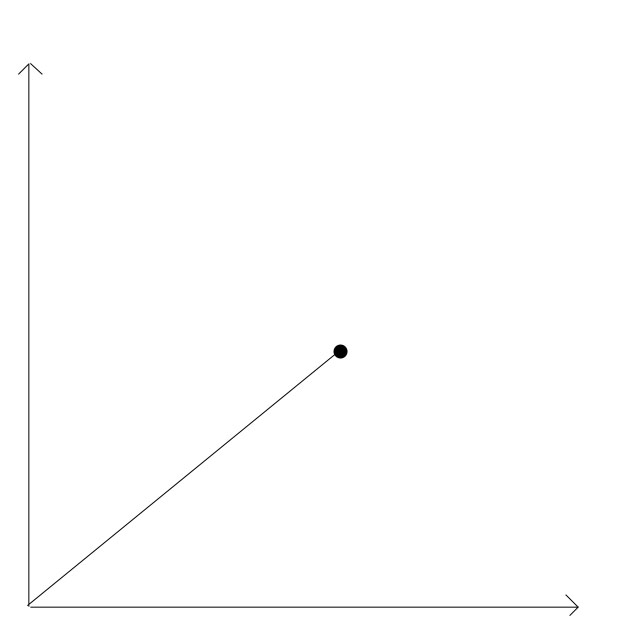
\includegraphics[scale=0.8]{LinAlgVec}
	
\end{figure}
		به برداری که مختصات افقی، یا عمودی آن، یک باشد بردار واحد میگویند. بردار واحد افقی را $ \vec{i} $ و بردار افقی عمودی را $ \vec{j} $ میگویند. بردار ها را میتوان به صورت مضربی از بردار واحد نشان داد مثلا بردار $ \vec{V} = \begin{pmatrix}
	X \\ Y
	\end{pmatrix}$ را میتوان به صورت $ X\vec{i} + Y\vec{j} $ نشان داد. 
	
	
	
	
یک بردار دارای دو خصیصه می باشد. \textbf{جهت}\footnote{Direction} و \textbf{مقدار}\footnote{Magnitude}. که به صورت زیر نشان داده میشود:

	
		 \begin{center}
		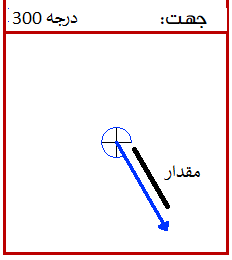
\includegraphics[scale=1]{DirMag}
	\end{center}

برای به دست آوردن مقدار بردار ازین فرمول استفاده میکنیم:
\[ |\vec{V}| =  \sqrt{x^2 + y^2} \]
	
	
	
	 
	 دو بردار را میتوان به صورت زیر جمع کرد:
	 
	 
	 	 \begin{center}
	 	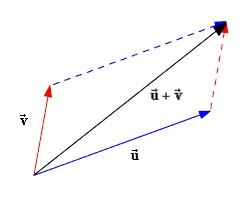
\includegraphics[scale=1]{VectorAdd}
	 \end{center}
 
 و به این صورت تفریق کرد:
  
 \begin{center}
 	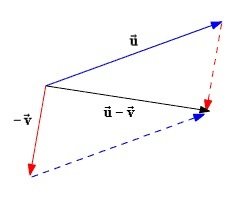
\includegraphics[scale=1]{VectorSubtract}
 \end{center}
 
	 
	 
	 اما دو نوع ضرب برداری داریم. \textbf{ضرب نقطه ای}\footnote{\lr{Dot Product}} و \textbf{ضرب صلیبی}\footnote{\lr{Cross Product}}. قبل ازین که پیش بروید، قسمت مثلثات \(\ref{trig}\) را بخوانید. فرض کنید دو بردار به صورت زیر هستند:
	 
	 
	  \begin{center}
	 	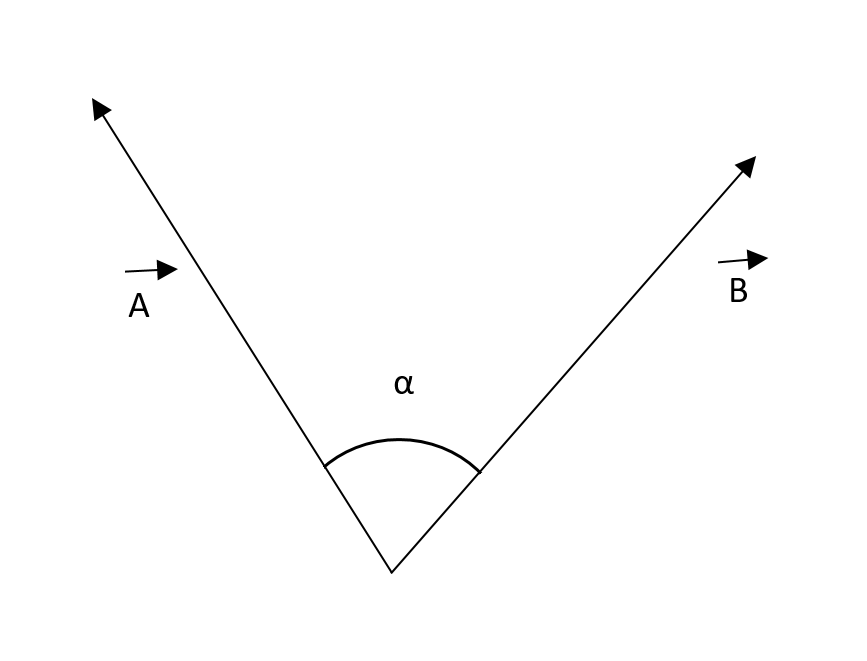
\includegraphics[scale=0.3]{Product}
	 \end{center}
	 
	 
	 ضرب نقطه ای به صورت زیر تعریف میشود:
	 
	 \[ \vec{A}.\vec{B} = |A||B|\cos \alpha \]
	 
	 و ضرب صلیبی ازین فرمول استفاده میکنیم.
	 \[ \vec{A} \times \vec{B} = |A||B|\sin \alpha \vec{n} \]
	 
	 
	 که  $\vec{n} $ برداری \textbf{پایه}\footnote{\lr{Basis Vector}}  عمود بر دو بردار است. برای به دست آوردن $\vec{n}$ کافیست از انگشتان وسط، اشاره، و شصت خود استفاده کنید. انگشت شصت شما، همواره بردار پایه ی عمود است، که مضربی از ضرب صلیبی دو بردار می باشد.
	 
	 
	 \section{مثلثات}\label{trig}
	 
	 مثلثات بحثیست پیپیده. و من نیز ریاضیدان نیستم پس به کمی در مورد این مبحث قناعت میکنیم.  قبل از هرچیزی، بگذارید در مورد \textbf{دستگاه مختصات قطبی}\footnote{\lr{Polar Coordinate System}} حرف بزنم. دستگاه مختصات قطبی، مانند دستگاه مختصات دکارتی، دارای دو محور عمودی و افقی است. اما در این دستگاه مختصات، ما یک نقطه را، عوض $ X $ و $ Y $ توسط یک زاویه $ \alpha $ و یک بردار شعاع $ \vec{r} $ نشان میدهیم:
	 
	 
	 
	 	  \begin{center}
	 	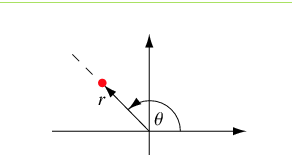
\includegraphics[scale=1]{Polar}
	 \end{center}
 
 در برنامه نویسی گرافیکی، دستگاه مختصات قطبی کاربردهای زیادی دارد. اما در کامپیوتر، \textbf{پیکسلها}\footnote{در مورد پیکسلها به وفور حرف خواهم زد.} در دستگاه مختصات دکارتی قرار دارند. حلال مشکلات ما، مثلثات است.
 یک دایره ی واحد را در دستگاه مختصات  قطبی کنید که شعاعش 1 میباشد:
  \begin{center}
 	\includegraphics[scale=1]{UnitCIrcle}
 \end{center}

اگر زاویه ی $   30\degree   $ را انتخاب کرده و یک مثلث قائم الزاویه دور آن بکشیم:


	   \begin{center}
	 	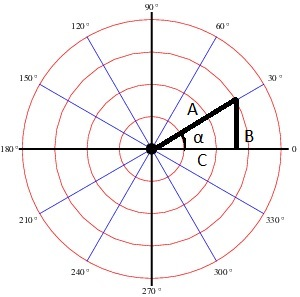
\includegraphics[scale=1]{ThirtyDegrees}
	 \end{center}
	 
	 سینوس و کسینوس زاویه 30 درجه که اینجا $ \alpha $ نامیده میشود، به صورت زیر تعریف میگردد:
	 \[ \sin \alpha = \frac{\text{مقابل}}{\text{وتر}} \]
	 
	 و:
	 
	 \[ \cos \alpha = \frac{\text{مجاور}}{\text{وتر}} \]
	 
	 همچنین تانژانت و کتانژانت به صورت زیر تعریف میشوند:
	 
	  \[ \tan \alpha = \frac{\sin \alpha}{\cos \alpha} \]
	  
	  
	  و 
	  \[ \cot \alpha = \frac{\cos \alpha}{\sin \alpha} \]
	  
	  
	  درجه، تنها واحد اندازه گیری زاویه نیست. واحد دیگر، \textbf{رادیان}\footnote{Radians} نام دارد. یک زاویه در رادیان، بین $ 0 $ و $   2\Pi $ قرار دارد. ارزش $ \Pi $ حدود $ 3.1415926535 $ است. ما برای کار با پیکسلها، ارقام اعشار بیشتر ازین نیز نیازمندیم. برای تبدیل درجه به رادیان:
	  \[ n\degree \times 	  \frac{\pi}{180} \]
	  
	  و بالعکس:
	  
	  \[ n \space \textrm{rad} \times 	  \frac{180}{\pi} \]
	  
	  
	  
	  
	  توابع مثلثاتی توسط \textbf{هویتهای مثلثاتی}\footnote{\lr{Trigonometric Identities}} به هم ربط داده میشوند. بعضی ازین هویتها عبارتند از:
	  
	  \[ \sin^2 \alpha + \cos^2 \alpha = 1 \]
	  \[ \sin(-\alpha) = -\sin\alpha \]
	  \[ \cos(-\alpha) = \cos(\alpha) \]
	  \[ \sin(\alpha\pm\beta) = \sin\alpha\cos\beta \pm\cos\alpha sin\beta \]
	  \[ \cos(\alpha\pm\beta) = \cos\alpha\cos\beta\pm\sin\alpha\sin\beta \]
	 
	 
	 اینها تقریبا تمام سرفصهلایی هستند که شما برای این کتاب لازم دارید. توجه کنید، این کتاب، نه برنامه نویسی گرافیکی و بازی سازی کلی.
	 
	 \section{ماتریسها}\label{matrix}
	 
	 به آرایه هایی از اعداد که به صورت n سطر و m ستون به نمایش در می آیند.، \textbf{ماتریس}\footnote{Matrix} میگویند. یک ماتریس را به این صورت نشان میدهند:
	 \[ A_{m, n} = \begin{bmatrix}
	  a_{1,1} & a_{1,2} & \cdots & a_{1,n} \\
	 a_{2,1} & a_{2,2} & \cdots & a_{2,n} \\
	 \vdots  & \vdots  & \ddots & \vdots  \\
	 a_{m,1} & a_{m,2} & \cdots & a_{m,n}
	 \end{bmatrix} \]
	 
	 
	 در ساخت بازیهای کامپیوتری و برنامه نویسی گرافیکی ما بیشتر نیاز به ماتریسهای $ 2\times2 $، $ 3\times3 $  و $ 4\times 4$ داریم.
	 
	 جمع و تفریق ماتریسها به صورت همسان انجام میشود:
	 
	 \[ A_{m, n}\pm B_{m, n} = \begin{bmatrix}
	 a_{1, 1} \pm b_{1, 1} && a_{1, 2} \pm b_{1, 2} && \cdots &&  a_{1, n} \pm b_{1, n} \\
	 a_{2, 1} \pm b_{2, 1} && a_{2, 2} \pm b_{2, 2} && \cdots &&  a_{2, n} \pm b_{2, n} \\
	 \vdots  && \vdots  && \ddots && \vdots \\
	 a_{m, 1} \pm b_{n, 1} && a_{n, {\tiny }2} \pm b_{n, 2} && \cdots &&  a_{m, n} \pm b_{m, n}
	 	
	 \end{bmatrix} \]
	 
	 ضرب ماتریسها به این روش صورت میپذیرد که، هر سطر با یک ستون. پس تا سطرها و ستونهای دو ماتریس با هم مساوی نباشند، ضرب صورت نمیپذیرد. مثلا ضرب دو ماتریس $ 2\times2 $ به صورت زیر است:
	 
	 \[ A_{2, 2}B_{2, 2} = \begin{bmatrix}
	 a_{1, 1} b_{1, 1} + a_{1, 2}  b_{2, 1} && a_{1, 1} b_{2, 1} + a_{1, 2}  b_{2, 2} \\
	 	a_{2, 1}  b_{1, 1} + a_{2, 2}  b_{2, 1} && a_{2, 1}  b_{2, 1} + a_{2, 2}  b_{2, 2}
	 \end{bmatrix} \]
	 
	
	 
	 
	

یکی دیگر از عملیتهای ماتریسی، \textbf{دترمینان}\footnote{Determinant} است. برای احتساب دترمینان ماتریسهای بزرگتر از  $ 3\times3 $ الگوریتمهای زیادی مانند \textbf{دیکامپوزیشن}\footnote{Decomposition} وجود دارد که خود آن توسط افراد مختلفی در طول سالها بهسازی گشته است، اما راه ساده ای برای به دست آوردن دترمینان $ 2\times2 $ وجود دارد که به شرح زیر است:

\[ A = \begin{bmatrix}
A && B\\ 
C && D
\end{bmatrix} \]
\[ |A| = AD - BC \]
	 
	 به $ I_{n} $ ماتریس \textbf{هویت} \footnote{Identity} میگویند و مثلا $ I_3 $ به صورت زیر تعری میشود:
	 
	 \[ I_{3} = \begin{bmatrix}
	 1 && 0 && 0 \\
	 0 && 1 && 0 \\
	 0 && 0 && 1
	 \end{bmatrix} \]
	 
	 ما در برنامه نویسی گرافیکی و بازی سازی از ماتریسها استفاده های زیادی خواهیم برد.
	 
	 \section{قائمیت در فضای سه بعدی}\label{r3}
	 
	 
	 ما در بخش بردار دیدیم که دستگاه مختصات دکارتی شامل دو محور عمودی و افقی است. اما همیشه اینگونه نیست، بلکه، میتوان با اضافه کردن یک بردار اضافه که نام آن $ Z $ است به دستگاه سه بعدی دست پیدا کنیم. این دستگاه را به صورت $ \mathbf{R^3} $ نشان میدهند و در تصویر زیر میتوانید محور $ Z $ را مشاهده کنید:
	  
	 
	\begin{figure}[h]
		\centering
		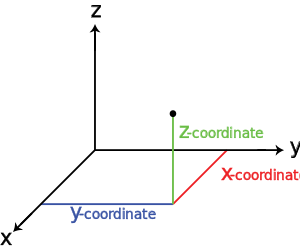
\includegraphics[scale=1]{R3}
	\end{figure}
	 
	 توجه کنید که در بعضی از نرم افزارها جای $  Y $ با $ Z $ عوض میشود.
	 
	یک بردار را در فضای $ R^3 $ به صورت زیر نشان میدهیم:
\[  \vec{V} = \begin{pmatrix}
X \\
Y \\
Z
\end{pmatrix}  \]
	 همه ی قوانین $ R^2 $ برای  $ R^3 $ برقرار است. مثلا به بردار واحد محور $ Z $، $ \vec{k} $ میگویند. غرض از این بخش، اینست که \textbf{قائمیت}\footnote{ Orthogonality} در فضای سه بعدی را معرفی کنم. زیرا برای بازیهای دو و نیم بعدی، دوربین باید قائم بر فضای $ R^3 $ باشد.
	 
	 

	 \begin{figure}[H]
	 	\centering
	 		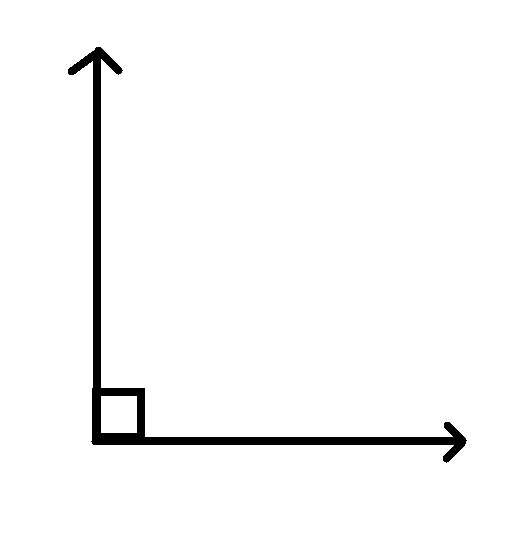
\includegraphics[scale=0.3]{Orthogonal}
	 \end{figure}

	 در کل، دو بردار وقتی بر هم قائمند که حاصلضرب نقطه ای آندو، صفر باشد:
	 \[ \vec{A} \text{قائم است بر } \vec{B} \text{اکر و تنها اگر} \vec{A}.\vec{B} = 0 \]  
	 
	 اگر فرمول ضرب نقطه ای یادتان باشد، و در اینترنت کسینوس 90 را خوانده باشید، میدانید که:
	 
	 
	 
	 \[ \vec{A}.\vec{B} = |A||B|\cos \alpha \]
	 
	 و $ \ cos(90)  = 0$
	 پس:
	 
	 \[ |A||B|\cos (90) = 0 \ \]
	 
	 
	 
	 \section{دنباله ها و سری ها}\label{seqserie}
	 
	 \textbf{دنباله}\footnote{Sequence} تابعیست به مانند زیر:
	 \[ f: \mathbb{N} \longrightarrow \mathbf{A} \]
	 که دامنه ی آن، اعداد طبیعی است. یک عضو در یک دنباله میتواند بینهایت تکرار شود. مثلا دنباله ی زیر:
	 \[ \frac{1}{2}, \frac{2}{3}, \frac{3}{4}, \frac{4}{5}, \frac{n}{n+1}, \]
	 یک دنباله ی \textbf{نامتناهی}\footnote{Infinite} \textbf{کراندار}\footnote{Convergent} میباشد. اگر بردِ دنباله، به عدد خاص نزدیک شود، کراندار و در در صورتی که به عددی خاص نزدیک نشود، بیکران است.  عضو n از دنباله ی A را $ a_n $ تعریف میکنیم و به آن \textbf{ایندکس}\footnote{Index} \lr{n} میگوییم.
	 دنباله ی \textbf{فیبوناچی}\footnote{Fibonacci} را به صورت زیر تعریف میکنیم:
	 \[ 1, 1, 2, 3, 4, 8, 13, 21, F_{n-1}+F_{n-2}, \]
	 
	 که یک دنباله ی نامتناهی بیکران است. 
	 
	 
	 \textbf{سری}\footnote{Series} توضیحاتی است که تعیین کننده ی بعلاوه کردن بینهایت یک سری اعداد است. برای نشان دادن سریها، از علامت جمع یعنی \textbf{سیگما}\footnote{Sigma} استفاده میکنیم:
	 \[  \sum_{n = 1}^{\infty} 2^n  \]
	 این جمله به ما میگوید: اول، n را 1 بگیر. بعد برای 1 تا بینهایت، 2 را به توان n برسان. حتما لازم نیست تا بینهایت باشد، یا اینکه از 1 شروع بشود.
	 
	 \[ \sum_{n = 3}^{8} n = 3+4+5+6+7+8 \]
	 
	 علامت $ \infty $ \textbf{بینهایت} نام دارد. بینهایت، عددی آنقدر بزرگ است که نمیتوانیم آنرا بشماریم. 
	 
\section{پایان فصل ریاضی}\label{mathend}

کلید یادگرفتن ریاضی یک چیز است: $  \text{تمرین}^n  $! یادتان نرود که حافظه، چیزیست فرَار، و هر لحظه ممکن است همین چیزهای کمی که از بنده ی حقیر آموخته اید، که مطمئنم برای بیشتر شما یک یادآوری ساده و کوتاه بوده، و برای خیل عظیمی از شما فوت آب بوده، و فقط یک لیست است، سریع از حافظه ی شما رخت برمیبندند. تمرین کنید، نوت برداری کنید، و یادتان نرود که روم را در یک روز نساخته اند. این ضرب المثال را چندین بار در طول کتاب تکرار خواهم کرد. یادگیری طول میکشد. و یادتان نرود که هیچکس استعداد چیزی را ندارد، و همه چیز با تمرین میسر میشود.

در فصل بعد، در مورد برنامه نویسی، زبان پایتان و \lr{C++} حرف خواهیم زد.
	 
	   
	 \chapter{نگاهی کوتاه به برنامه نویسی}\label{programming}
	 
	 درین فصل نگاهی کوتاه می اندازیم به \textbf{برنامه نویسی}\footnote{Programming}. ابتدا به دو \textbf{پَرَدایم}\footnote{Paradigm} برنامه نویسی \textbf{فانکشنال}\footnote{Functional} و \textbf{شیء گرا}\footnote{\lr{Object Oriented Programming}}. بعد از آن، نگاهی می اندازیم به \textbf{سینتکسِ}\footnote{به دستور زبانی یک زبان برنامه نویسی Syntax گفته میشود.} زبان \textbf{پایتان}\footnote{Python} و \textbf{\lr{C++}}.
	 
\section{برنامه نویسی فانکشنال}\label{functional}

از بین تمام روشها، یا به عبارتی، پَرَدایمهای برنامه نویسی، برنامه نوسی فانکشنال یا \textit{تابعی} ساده ترین، و پر مصرف ترین آنهاست. اکثر اشخاصی که برنامه نویسی را شروع میکنند، از برنامه نویسی فانکشنال شروع میکنند. زبانهای قدیمی مانند \textbf{فورترن}\footnote{FORTRAN}	و \textbf{لیسپ}\footnote{Lisp} همه فانکشنال هستند. 

با توابع در فصل ریاضی آشنا شدیم. توابع کامپیوتری نیز با توابع ریاضی فرق زیادی ندارد، همه ی آنها یک ماشین هستند که ورودی را به خروجی تبدیل میکنند. یک تابع، مجموعه ای از \textbf{دستورات}\footnote{Instructions} است که \textbf{پارامتر}\footnote{Parameter} داده شده را با تغییرات، باز میگردانند. این تغییرات میتواند عملیاتهای جمع و تفریق، ضرب و تقسیم، باقیمانده، و یا تغییر نوع پارامتر مثلا از عدد صحیح به عدد حقیقی، و یا هرچیز دیگری باشد. برای اجرای تابع، آنرا \textbf{میخوانیم}\footnote{Call} و به پارامتری که به آن میدهیم، \textbf{آرگومان}\footnote{Argument} میگوییم.

اینستراکشن سِت زیر را در نظر بگیرید:

\begin{enumerate}
	\item عدد $ n $ را بگیر.
	\item برای $ n $ بار، $ n $ را ضربدر $n - 1$ کن.
	\item جواب را برگردان.

\end{enumerate}

به این تابع، تابع \textbf{فاکتوریل}\footnote{Factorial} میگویند. توابع زیادی هستند، پیچیده و ساده، مهم اینجاست که از آنها درست استفاده کنید. 
بعضی از توابع، پارامتر قبول نمیکنند. بعضی از توابع، ارزشی را باز نمی گردانند. به این نوع از توابع \textbf{ووید}\footnote{Void} میگویند. بعضی از زبانها، \textbf{تایپ ثابت}\footnote{\lr{Statically Typed}} هستند و باید نوع ارزشهای باز گرداننده را مشخص کرد. \lr{C++} یکی ازین نوع زبانهاست. بعضی از زبانها \textbf{تایپ دینامیک}\footnote{\lr{Dynamically Typed}} هستند و لازم نیست نوع ارزش بازگرداننده را در آنها مشخص کرد. پایتان یکی ازین زبانهاست. هردو زبان پایتان و \lr{C++} هم فانکشنال هستند، هم شیء گرا. در مورد پَرَدایم شیء گرا در بخش بعد صحبت خواهیم کرد. 
هرزبان مقداری تابع از پیش  شده دارد، اما بقیه ی تابع ها را خودتان باید تعیین کنید. اینکه در چه زمانی باید تابع تعیین کرد، قانون طلایی اینست که هرگاه دیدید عملی را دارید بیشتر از یک بار انجام میدهید، وقت تعیین کردن یک تابع است. 
همه ی زبانها دارای \textbf{کتابخانه}\footnote{Library} هایی هستند که شامل توابع و کلاسها \(\ref{oop}\) و دیگر کدهایی هستند که به برنامه نویس کمک میکنند خود را تکرار نکند.
 
	 
	\textbf{خود را تکرار نکنید.}\footnote{\lr{DRY - Don't Repeat Yourself}}
	
	قانون پلاتینیوم برنامه نویسی، اینست. هرگز چیزی که در یک کتابخانه موجود است را ننویسید. مثلا عوض اینکه در زبان \textbf{جاوا}\footnote{Java} عوض نوشتن صدها خط کد برای به دست آوردن یک تابع ماتریس، میتوان از کتابخانه ی JAMA استفاده کرد.
	
	
	
	
	
	
	 
	 \section{برنامه نویسی شیء گرا}\label{oop}
	 
	 
	 برنامه نویسی شیء گرا بر پایه ی کانسپتِ \textbf{کلاس}\footnote{Classes} میجرخد.
	 
	 گفتیم توابع مانند ماشینهایی هستند که اطلاعات را از حالتی به حالت دیگر تغییر میدهند. اگر تابع، ماشین است، کلاس، یک خیابان پر از ماشین است که در آن هزاران ماشین وجود دارد، و همچنین چندده هزار عابر پیاده که سوار ماشین میشوند. درین تشبیه، به ماشین \textbf{اسلوب}\footnote{Method} و به عابر پیاده \textbf{خواص}\footnote{Properties} میگویند. اگر ایده ی کلاس، یعنی یک خیابان پر از عابر پیاده و ماشین \(به ترتیب، اسلوب و خواص\) را داشته باشیم، با آن میتوانیم هزاران هزار خیابان بسازیم. به هر خیابانی که ما میسازیم، \textbf{شیء}\footnote{Object} میگویند. مثلا خیابان ولیعصر، یک شیء خیابان است. در یک کتابخانه مانند کتابخانه ی JAMA که از آن نام بردیم، یک کلاس به نام ماتریس وجود دارد و این کلاس چندین اسلوب و چندین خواص دارد. یکی از آن اسلوبها، ارزش سطر و ستون داده شده را به کاربر برمیگرداند.
	 
	 بعضی از متدها و خواصها، خصوصی اند، یعنی جز سازنده ی کلاس خیابان، کسی اجازه ی عوض کردن آن را ندارد. اما بعضی از اسلوبها و متدها قابل تغییرند.
	 
	 یک کلاس میتواند فرزند یک کلاس دیگر باشد. در بعضی از زبانها، یک کلاس میتواند فرزند چندین کلاس باشد. \lr{C++} یکی ازین زبانهاست.
	 
	 فرض کنیم یک کلاس داریم به نام مدرسه. برای ساختن یک شیء مدرسه از آن، باید به آن \textit{ارزشهایی} مانند آدرس مدرسه، تعداد کلاسها، اینکه مدرسه بوفه داشته باشد یا نه، نام مدرسه، اینکه دبیرستان است یا ابتدایی، و... را بدهیم تا از آنها، \textit{خواص} مدرسه را تعیین کند. این کار توسط اسلوب \textbf{سازنده} \footnote{Constructor} انجام میشود. و یا به سادگی میخواهیم یک مدرسه ی قدیمی را بکوبیم و خراب کنیم. برای این کار از اسلوبی به نام \textbf{خراب کننده}\footnote{Destructor} استفاده میکنیم. 
	 یگ کلاس میتواند چنین سازنده داشته باشد، ولی فقط یک خراب کننده میتواند داشته باشد.
	 
	 در بخش بعدی در مورد کتابخانه ها صحبت خواهیم کرد.
	 
	 \section{کتابخانه ها}\label{lib}
	 
	 به مجموعه توابع و کلاسهای از قبل آماده شده، کتابخانه میگویند.
	 
	 هر کدی که در صورت اجرا، عملیات خاصی انجام نداده، و به کدهای دیگر برای اجرا وابسته باشد، کتابخانه نام میگیرد.
	 اکثر زبانها برای کتابخانه های خود دارای یک دیتابیس هستند، که زبان پایتان جزء آنهاست، اما بعضی از زبانها برای کتابخانه های خود دیتابیس ندارد، مانند \lr{C++}. دلیل آن اینست که اکثر کتابخانه های \lr{C++}، متن بسته و پولی هستند.
	 
	 کتابخانه ها میتوانند به صورت فایل متنی، یا فایل \textbf{باینری}\footnote{Binary} عرضه شوند. کتابخانه های پایتان متنی، و کتابخانه های \lr{C++} باینری هستند. گاها کتابخانه هایی به صورت متنی نیز عرضه میشوند.
	 
	 
	 \section{پایتان}\label{py}
	 
	 زبان پایتان در سال 1999 برای بار اول عرضه شد و در هنگام نوشتن این کتاب، در ورژن 1.7.3 به سر میبرد. درین فصل، فقط قطره ای از دریای این زبان را آموزش میدهیم. برای آموزش بهتر زبان، به کتاب مخصوص مراجعه کنید.
	 
	 پایتان زبانی کاملا مدرن، قابل انعطاف، یکدست، و جذاب و ساده میباشد که برای از اتوماسیون گرفته تا بازی سازی، کاربرد دارد. 
	 اینستراکشن های پایتان \textbf{ترجمه}\footnote{Interpret} میشوند، یعنی لازم نیست که از قبل به زبان اسمبلی یا ماشین در بیایند، بلکه، در حین اجرا به زبانهایی مثل C یا Java ترجمه میشوند و بعد خط به خط اجرا میشوند. عرضه ی اصلی پایتان که ما از آن استفاده میکنیم، از \lr{C++} استفاده میکند.
	 
	\subsection{نصب پایتان}\label{pyinstall}
\begin{enumerate}
	\item به این صفحه بروید و پایتان را دانلود کنید: \url{https://www.python.org/downloads/}
	\item آنرا نصب کنید.
	\item از فایل اکسپلورر مانند زیر روی Properties کلیک کنید:
		 \begin{center}
		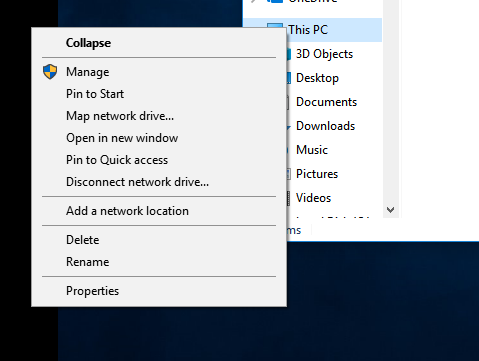
\includegraphics[scale=1]{InstallPython_1}
	\end{center}
	\item  روی \lr{Advanced System Settigns} کلیک کنید.
	\begin{center}
		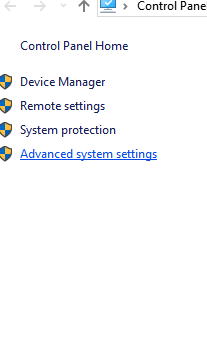
\includegraphics[scale=1]{InstallPython_2}
	\end{center}
\item روی گزینه \lr{Environment Variables} کلیک کنید.
\begin{center}
	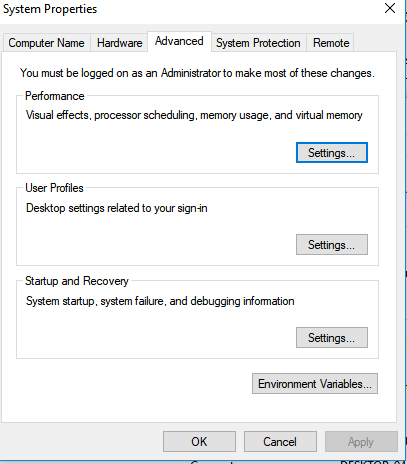
\includegraphics[scale=1]{InstallPython_3}
\end{center}
\item روی Path  کلیک کنید.
\begin{center}
	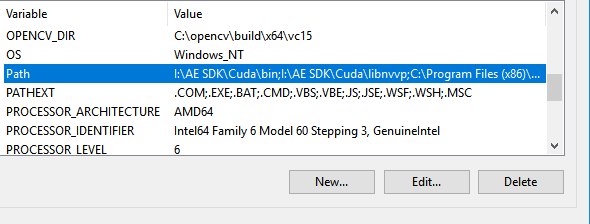
\includegraphics[scale=1]{InstallPython_4}
\end{center}
\item دو گزینه ی زیر را به آن اضافه کنید.
\begin{center}
	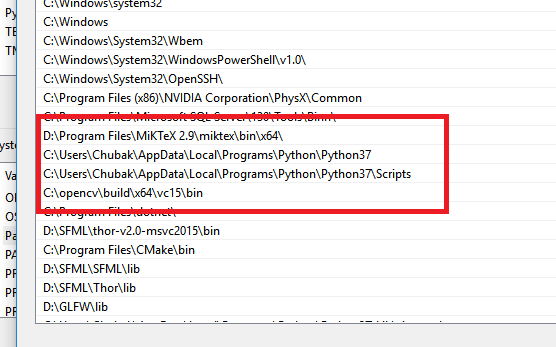
\includegraphics[scale=1]{InstallPython_5}
\end{center}
\end{enumerate}
	 
	 برای نوشتن کد پایتان احتیاج به یک \textbf{محیط گسترش مجتمع]}\footnote{Integrated Development Environment} دارید. من \lr{PyCharm Community} را پیشنهاد میکنم که کاملا مجانیست. آنرا میتوانید از \url{https://www.jetbrains.com/pycharm/download/#section=windows} دانلود کنید. 
	 بعد از باز کردن پای چارم و باز کردن یک پروژه ی جدید، از طریق زیر یک فایل پایتان بسازید:
	 
	 \begin{center}
	 	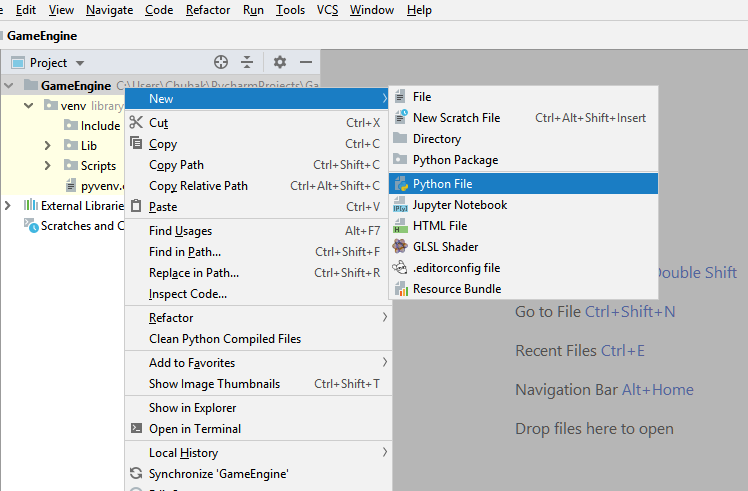
\includegraphics[scale=0.6]{CreateNewPythonFile}
	 	\end{center}
 	
 	حال وقت نوشتن اولین کد ماست. بنویسید:
 	
 	
 	\begin{latin}
 	\mono{	\begin{lstlisting}[backgroundcolor = \color{lightgray}]
new_variable = "A Portal to the World of Python"
print(new_variable)
 		\end{lstlisting}}
 	
 \end{latin}
و \lr{\keys{\ctrl + \shift + F10}}  را بزنید. در پایین صفحه، کد شما اجرا میشود.
\begin{tip}
	میتوانید از محیطهای گسترش دیگر نیز استفاده کنید. مانند \lr{Beans IDE}، PyDev، SpyDer، \lr{Cloud9 IDE}و درضمن، \lr{Microsoft Visual Studio} نیز یک پکیج پایتان دارد.
\end{tip}


	 
	 
	 
	 \subsection{متغیرها}\label{vars}
	 در بخش قبل، \lr{\mono\lstinline|new_variable|} یک \textbf{متغیر}\footnote{Variable} است. ممتغیرها مانند ظروفی هستند که میتوان در آنها هر چیزی ریخت. چون پایتان زبان \textbf{تایپ امن}\footnote{\lr{Type Safe}} \textit{نیست}، میتوان هر نوع دیتایی را داخل یک متغیر جا داد.
	 
	 
	 	\begin{latin}
	 		
	 	\mono{	\begin{lstlisting}[backgroundcolor = \color{lightgray}]
var = True #boolean
var = "String" #string
var = 1 #integer
var = 1.0 #float	
var = Class() #Class
	 		
	 		
	 		\end{lstlisting}} \end{latin}
	 
	 همانطور که میبینید، متغیرهای پایتان هر \textbf{نوع دیتایی }\footnote{دیتا تایپ} را قبول میکنند، استرینگ، عدد صحیح، فلوت و کِلس. بگذارید تمام این انواع دیتا را توضیح دهم.
	 
	 \begin{itemize}
	 	\item به متغیرهایی که دو حالت \textbf{راست}\footnote{True} و \textbf{غلط}\footnote{False} دارند، متغیر \textbf{بولی}\footnote{Boolean} میگویند.
	 	\item به تکه های متنی که از الفباء تشکیل شده، \textbf{رشته} یا String میگویند. به متنی که به یک استرینگ میدهیم، \textbf{لیترال}\footnote{Literal} میگویند.
	 	\item  به اعداد صحیح بدون اعشار \textbf{اینتجر}\footnote{Integer} یا به کوتاه int میگویند.
	 	\item به عدد حقیقی با اعشار \textbf{فلوت}\footnote{Float} میگویند
	 	\item از هر کلاسی می توان یک متغیر ساخت. درین صورت، نام کلاس، نوع متغیر میشود.
	 \end{itemize}
 
 اینها فقط چند نوع از متغیرهای پایتان هستند. همانطور که گفته شد، لازم نیست نوع متفیر را مشخص کنید چون پایتان، تایپ امن نیست. اما لازم است برای تعیین نوع آن، آنرا \textbf{مقداردهی اولیه}\footnote{Initialize} نمایید.
	 
	 
	اما اگر بخواهیم چندین نوع دیتا، یا متغیر، را در یک متغیر نگاه داریم چه؟ بخش \ref{list} درین مورد صحبت خواهد کرد.
	
	\subsection{لیست، تاپل، دیکشنری}\label{list}
	 
	 برای نگاه داشتن چندین نوع دیتا، یا چندین متغیر، در یک مکان، از \textbf{لیست}\footnote{Lists} استفاده میکنیم.لیستها به صورت زیر مقداردهی اولیه میشوند:
	 
	  	\begin{latin}
	 	\mono{	\begin{lstlisting}[backgroundcolor = \color{lightgray}]
a_list = []
a_list = [1, 2, 3, 4]
a_list = ["Hello World", "Goodbye World"]
a_list = [1, 2, 3, 4, "Hello", "World"]
	 		\end{lstlisting}}
	 	
	 	\end{latin}
	 		
	 		یک لیست وقتی مقداردهی اولیه شد، نباید با علامت مساوی، به آن مقدار اضافه کرد. بلکه، باید از \lr{\mono\lstinline|list.append|} استفاده کرد:
	 	\begin{latin}
	 	\mono{	\begin{lstlisting}[backgroundcolor = \color{lightgray}]
a_list = [1]
print(a_list)
a_list.append(2)
print(a_list)
	 		\end{lstlisting}}
	 			
	 	\end{latin}
 		
 \lr{\keys{\ctrl + \shift + F10}} را بزنید تا نتیجه را ببینید.
 		در زیر چند اسلوب لیست را میخوانید.
 		\begin{itemize}
 			\item \lr{\mono\lstinline|list.reverse|}: لیست را برعکس یا به بعیارت دیگر، معکوس میکند.
 			\item  \lr{\mono\lstinline|list.copy|} لیست را در لیست دیگر کپی میکند.
 			\item  \lr{\mono\lstinline|list.pop|} در \textbf{ایندکس}\footnote{Index - به شماره ی عضو ایندکس میگویند.} داده شده، عضو را پاک میکند.
 			\item \lr{\mono\lstinline|list.sort|} لیست را بر اساس الگوریتم \textbf{\lr{Merge Sort}} مرتب میکند.
 			\item  \lr{\mono\lstinline|len(list)|} سایز لیست را به دست می اورد.
 		\end{itemize}
 		
	 		
	 یک لیست، میتواند لیستهای دیگری نیز در بر بگیرد:
	 
	 
	 	\begin{latin}
	 	\mono{	\begin{lstlisting}[backgroundcolor = \color{lightgray}]
multi_dimensional_list = [[], [], []]
multi_dimensional_list.append([])
	 		\end{lstlisting}}
	 	
	 \end{latin}
 
 برای به دست آوردن عضو خاصی از لیست، از ایندکس آن استفاده میکنیم.
 
 	 	\begin{latin}
 	\mono{	\begin{lstlisting}[backgroundcolor = \color{lightgray}]
 my_list = [2, 4, 6, 8, 10]
 print(my_list[0])
 		\end{lstlisting}}
 	
 \end{latin}
\textbf{ایندکسها از 0 شروع میشوند} تا سایز لیست منهای یک ادامه دارند. برای بدست آوردن چندین عضو از لیست، از علامت دو نقطه استفاده میکنیم:

 	 	\begin{latin}
	\mono{	\begin{lstlisting}[backgroundcolor = \color{lightgray}]
my_list = [2, 4, 6, 8, 10]
print(my_list[0:3])
		\end{lstlisting}}
	
\end{latin}

 	 
	 در کل، لیستها بهترین روش برای نگه داشتن دیتاهای زیاد هستند. اما برای دیتای کم و \textbf{غیر جهشی}\footnote{Immutable}، از \textbf{تاپل}\footnote{Tuple} استفاده میکنیم.  تاپلها میتوانند به اندازه ی لیست دیتا نگه دارند، اما نمیتوان از آنها دیتا کم و زیاد کرد. تاپلها بدین صورت تعریف مقداردهی اولیه میشوند:
	 
	 
 	 	\begin{latin}
	\mono{	\begin{lstlisting}[backgroundcolor = \color{lightgray}]
my_tuple = (R, G, B)
print(my_tupe[0:1])
		\end{lstlisting}}
	
\end{latin}
	 مقلا برای رنگ یا موقیت یک فرگمنت در یک تصویر رَستر \(در مورد اینها مفصل صحبت خواهیم کرد\) از تاپل استفاده میشود. مانند لیستها، میتوان از \lr{\mono\lstinline|len()|} برای بدست آوردن سایز تاپل استفاده کرد.
	 
	 دیکشنریها نیز مانند لیستها، برای نگه داشتن مقدار زیادی دیتا استفاده میشود. اما در دیکشنری، ایندکسها، عوض شماره، دارای نام هستند \(میتوان از شماره نیز استفاده کرد\). دیکشنریها \textbf{همتا به همتا}\footnote{Peer to Peer} هستند. برای مقداردهی اولیه ی یک دیکشنری، از تفریق زیر استفاده میکنیم:
	 
	 \begin{latin}
	 	\mono{	\begin{lstlisting}[backgroundcolor = \color{lightgray}]
my_dict = {"Name" : "Chubak",
	"Last Name" : "Bidpaa"}
print(my_dict["Name"])
	 	\end{lstlisting}}
	 	
	 \end{latin}
	 
	 \begin{tip}
	 	در تمام زبانهای برنامه نویسی، زدن \keys{\return}  وسط خط کد اشکالی ندارد.
	 \end{tip}
	 
	 
	 مهمترین اسلوب دیکشنری \lr{\mono\lstinline|dictionary.items()|} میباشد که آیتم های دیکشنری را برمیگرداند. در بخش لوپ در موردش صحبت خواهیم کرد صحبت از لوپ شد، وقت آن است که در مورد \textbf{بیانیه های}\footnote{Statements} پایتان صحبت کنیم.
	 
	 \subsection{بیانیه های شرطی}\label{pyif}
	 
	 
	 \textbf{بیانیه های شرطی}\footnote{\lr{Conditional Statements}}، بخشهایی از پایتان هستند که به کد اجازه ی اجرا، یا در صورت عدم اجازه، اجازه ی اجرای کد دیگری را میدهند.
	 
	 \textbf{کلمات کلیدی}\footnote{Keywords} که ما برای شرط گذاشتن روی جریان اجرای برنامه استفاده میکنیم، \textbf{if} و \textbf{else} و \textbf{elif} هستند. همیشه لازم نیست از دوتای دوم استفاده کرد، اما پیشنهاد میشود اگر مستلزم است، حتما از آنها استفاده کنید. کد زیر را ببینید:
	 
	 
	 \begin{latin}
	\mono{	\begin{lstlisting}[backgroundcolor = \color{lightgray}]
pi = 3.14
r = 10
area= pi*r*r
		
if area > 20:
	print("The area is greater than 20.")
else:
	print("The area is not greater than 20.")
		
		\end{lstlisting}}
	
\end{latin} 
	 
	این کد، مساحت یک دایره با شعاع 10 را حساب میکند و  اگر این مساحت، بیشتر از 20 است، میگوید مساحت بیشتر از 20 است، وگرنه میگوید مساحت بیشتر از 20 نیست. به همین سادگی، ما \textbf{جریان}\footnote{\lr{Execution Flow}} اجرای کد را تغییر دادیم. 
	
	\begin{tip}
		پای چارم خودش اینکار را میکند، اما بین اول خط کلمه ی if و else و \textbf{اصطلاح}\footnote{Expression} شرط، باید چهار \keys{\space} فاصله باشد.
	\end{tip}


برای شرط گذاشتن، از \textbf{آپریتور}\footnote{Operator} هایی مانند $ < $ استفاده میکنیم. به اعدادی که آپریتور روی آنها تاثیر میگذارد، \textbf{آپرَند}\footnote{Operand} میگویند.

آپریتور های شرطی پایتان به شرح زیرند:
	 
	 
	
	\begin{table}[H]\label{pyop}
		\centering
		\begin{tabular}{|l|l|}
			\hline
			+               & بعلاوه       \\ \hline
			-               & منها         \\ \hline
			*               & ضرب          \\ \hline
			/               & تقسیم        \\ \hline
			\%              & باقیمانده    \\ \hline
			\textgreater{}  & بزرگتر       \\ \hline
			\textless{}     & کوچکتر       \\ \hline
			\textgreater{}= & بزرگتر مساوی \\ \hline
			\textless{}=    & کوچکتر مساوی \\ \hline
			==              & مساوی        \\ \hline
			!=              & نامساوی     \\ \hline
			and             & وَ           \\ \hline
			or              & یا           \\ \hline
			!				& نیست \\ \hline
		\end{tabular}
		\caption{آپریتورهای پایتان}
	\end{table}
			


	 
	 
	 آپریتورهای دیگری نیز داریم مانند آپریتورهای \textbf{Bitwise} ولی الان به کار ما نمی آیند.
	 
	 میتوانید از کلمه ی کلیدی elif که مخفف Else If است برای افزایش شروط استفاده کنید:
	 
	 
	 \begin{latin}
	\mono{	\begin{lstlisting}[backgroundcolor = \color{lightgray}]
if area > 20:
	 print("The area is bigger than 20.")
elif area < 15:
	 print("The area is less than 15")
elif area < 10:
	 print("The area is less than 10")
else:
	 print("The area is not bigger than 20.")
	
		
		\end{lstlisting}}	 
	 
\end{latin}

اما این فقط تنها بیانه ی شرطی پایتان نیست. دو بیانیه ی شرطی دیگر داریم، که با if فرق زیادی دارند.



\begin{tip}
	شرط، میتواند یک متغیر بولی باشد. مثلا \lr{\mono\lstinline| bool = 1 < 10|}. این متغیر، راست $\text{(True)}\ $ میباشد چون 1 کوچکتر از 10 است.
\end{tip}


\subsection{بیانیه های چرخشی شرطی}\label{pyloops}
	 
	 بیانیه های \textbf{چرخشی شرطی}\footnote{\lr{Conditional Loops}} بیانیه هایی هستند که تا شرط برقرار است، یک اصطلاح یا بیانیه را به صورت \textbf{نا محدود}\footnote{Indefinitely} اجرا میکنند. گاهی این چرخش، بینهایت است. اما اکثر اوقات، شرط تمام شده و \textit{غلط} $\text{(False)}  $میشود. وقتی شرط، غلط میشود، چرخش تمام شده و بیانیه ی بعدی اجرا میشود. همچنین میتوانیم خودمان جریان چرخش را کنترل کرده، و به میل خود چرخش را تکرار کرده و یا بشکنیم.
	 
	 دو کلمه ی کلیدی برای اینکار استفاده میشود، for و while. اولی مصارف دیگری هم دارد که به آن میپردازیم. اما بگذارید اول به while بپردازیم. سینتکس آن اینگونه است:
	 
	 
	 
	 
	 \begin{latin}
	\mono{	\begin{lstlisting}[backgroundcolor = \color{lightgray}]
i = 0
		
while i < 50:
	print(str(i))
	i += 1
		
		\end{lstlisting}}	 
	
\end{latin}
	 
	 
	ابتدا ما به متغیر  \lr{\mono\lstinline|i|} عدد 0 را میدهیم. بعد میگوییم تا این متغیر، از 50 کوچکتر از، ارزش متغیر را روی صفحه نمایش بده و در هر \textbf{بازتکرار}\footnote{Iteration}، ارزش 1 را به متغیر اضافه میکنیم. وقتی متغیر به 50 رسید، چرخش تمام میشود و به بیانیه ی بعدی میرسد. 
	
	\begin{tip}
	تابع \lr{\mono\lstinline|print()|} نمیتواند جز استرینگ لیترال و استرینگ، چیز دیگری را در صفحه به نمایش بگذارد. با استفاده از تابع  \lr{ \mono\lstinline|str()| } متغیرهای عددی را به استرینگ لیترال تبدیل میکنیم.
	\end{tip}
	 
	 
	 
	 
	 میتوانید با استفاده از کلمه ی کلیدی \lr{\mono\lstinline|and| } یک شرط دیگر اضافه کنید:
	 
	 \begin{latin}
	\mono{	\begin{lstlisting}[backgroundcolor = \color{lightgray}]
i = 0
		
while i < 50 and i < 25:
	print(str(i))
	i += 1
		
		\end{lstlisting}}	 
	
\end{latin}
	 
	 
	 اینگونه، فقط در صورتی متغیر روی صفحه پرینت میشود که بین 25 و 50 باشد. \lr{\mono\lstinline|or|} هم دو یا چند شرط را در صورتی اجرا میکند که یکی از آنها، راست باشد. 
	 
	 کلمه ی کلیدی بعدی که داریم، for میباشد. این کلمه بیشتر برای دسترسی به لیست، دیکشنری و تاپل به کار میرود \(\ref{iter}\) اما برای چرخش برای n بار از سینتکس زیر استفاده میکنیم:
	 
	 
	 
	 
	 	 
\begin{latin}
	 	\mono{	\begin{lstlisting}[backgroundcolor = \color{lightgray}]
for i in range(n):
	print(str(i))
	 		
	 		\end{lstlisting}}	 
	 	
	 \end{latin}
	 
	 
	 
	 تابع  \lr{\mono\lstinline|range(m, n)|} یک لیست قابل بازتکرار بین m و n ایجاد میکند. اگر پارامتر اول را به آن ندهیم، یک لیست قابل بازتکرار بین 0 و n ایجاد میکند. و متغیر ارزش i را در هر بازتکرار، بر اساس لیست ساخته شده مشخص میکند. این بیانیه ی چرخشی شرطی نیست، بلکه بیانیه ی چرخشی بازتکراریست. در بخش بعد، از کلمه ی کلیدی for برای دسترسی به اعضای لیست، تاپل، و دیکشنری استفاده میکنیم.
	 
	 
\subsection{دسترسی به لیست، دیکشنری و تاپل}\label{iter}
	 
	 برای دسترسی به اعضای یک لیست، تاپل، دیکشنری، یا هر شیء \textbf{قابل بازتکرار}\footnote{Iterable} دیگری، از for استفاده میکنیم. مثال برای لیست اینگونه است:
	 
	 \begin{latin}
	 	\mono{	\begin{lstlisting}[backgroundcolor = \color{lightgray}]
one_dim_list = [1, 2, 3]
two_dim_list = [[1, 2, 3], [4, 5, 6]]
	 		
for i in one_dim_list:
	  print(i)
	 		
	 		
for list in two_dim_list:
	 for i in list:
	     print(i)
	 		\end{lstlisting}}	 
	 	
	 \end{latin}
	 
	 
	 
	 
	 همانطور که مشاهده میکنید، ما با استفاده از کلمه ی کلیدی in توانستیم به اعضای لیست یک بعدی \lr{\mono\lstinline|one_dim_list|} دسترسی پیدا کنیم و آنها را روی صفحه پرینت کنیم. سپس، ما با استفاده از یک بیانیه ی \textbf{لانه ای}\footnote{\lr{Nested Statement}} توانستیم یک لیست دو بعدی را روی صفحه پرینت بگیریم.
	 
	 \begin{tip}
	 	تمام بیانیه های چرخشی را میتوان لانه کرد، اما اگر که اشتباهی صورت بگیرد، \textbf{سرریزی پشته}\footnote{\lr{Stack Overflow}} صورت میپذیرد. پشته بخشی از زبان C است که کامپایلر پایتان در آن نوشته شده است.  \ref*{refpointer} را بخوانید.
	 \end{tip}
	 
	 
	 ما میتوانیم با استفاده از دو کلمه ی کلیدی break و continue بر جریان چرخشمان تاثیر بگذاریم.
	 
	 

		 	 \begin{latin}
			\mono{	\begin{lstlisting}[backgroundcolor = \color{lightgray}]
n = 0
while True:
	n += 1
				
	if (n > 20):
		break;
				\end{lstlisting}}	 
			
		\end{latin}

	 
	 
	 این کد، همیشه صحیح است، پس همواره اجرا میشود. اما اگر متغیر ما، بیشتر از 20 شود، زنجیر میشکند و چرخش پایان میابد. continue نیز مانند break است، فقط حلقه را نمیشکند، بلکه کاری میکند که حلقه دوباره بازتکرار شود.
	 
	 
	 
	\subsection{تابع در پایتان}\label{pyfunc}
	در بخش پَرَدایم فانکشنال، در مورد توابع در برنامه نویسی صحبت کردیم. در پایتان، تابع بلوکه ای از کد است که با خواندن آن، یک یا یک امر صورت میپذیرد، یا یک ارزش باز گردانده میشود، یا هردو. پایتان دارای 68 تابع از پیش ساخته شده است، و ما خودمان میتوانیم تا هرچقدر لازم داریم، تابع بسازیم. برای اینکار، از کلمه ی کلیدی def استفاده میکنیم:
	 
	 
	 \begin{latin}
	\mono{	\begin{lstlisting}[backgroundcolor = \color{lightgray}]
def first_functions():
	pi = 3.14
	r = 10
	area = pi * r * r
		
	print(area)
		
		
	def second_function(r):
	   pi = 3.14		    
	   area = pi * r * r
		
	   return area
		\end{lstlisting}}	 
	
\end{latin}


	 
همانطور که مشاهده میکنید، تابع اولی، نه پارامتر قبول میکند، نه ارزشی را باز می گرداند. اما یک عملیات پرینت انجام میدهد. به این نوع توابع، همانطور که گفتیم، ووید میگویند.

تابع دوم یک تابع فلوت است، چون یک ارزش فلوت باز می گرداند. و ابتدا شعاع دایره را به عنوان پارامتر میپذیرد.

یک تابع را میتوان در خودش بخواند. به این امر \textbf{تابع بازگشتی}\footnote{\lr{Recursive Function}} میگویند. مثلا برای بدست آوردن فاکتوریل یک عدد:



	 
	 
	 \begin{latin}
	\mono{	\begin{lstlisting}[backgroundcolor = \color{lightgray}]
def factorial(n):
	if n == 1:
	 return n
     else:
	 return n*factorial(n - 1)
		\end{lstlisting}}	 
	
\end{latin}
	 
	 
	 اگر شرایط بازگشت در تابع محیا نباشد همانطور که در بخش قبل گفتیم، سرریزی پشته صورت میگیرد. در مورد پشته و هرم در بخش \lr{C++} صحبت خواهیم کرد. تا این حد بدانید که پایتان، \textbf{مدیریت حافظه}\footnote{\lr{Memory Management}} را خودش انجام میدهد و نیازی به این کار توسط شما نیست. در \lr{C++} ما متغیرهایی داریم که به آدرس یک متغیر دیگر در RAM اشاره دارند، اما در پایتان، ما همچین چیزی نداریم.
	 
	 \begin{tip}
	 	توجه داشته باشید که \textbf{اسکوپ}\footnote{Scope} متغیرها در تابع، مخصوص خودشان است. اگر متغیری را در یک تابع تعیین کردید، نمیتوانید آنرا بیرون از تابع استفاده کنید. و همچنین اگر متغیری را داخل یک بلاک بیانیه ی شرطی یا چرخش شرطی تعیین کردید، آن متغیر، بیرون از آن بلاک، ارزشی ندارد.
	 \end{tip}	 
	 
	 
	 \subsection{فایل در پایتان}\label{pyfile}
	 برای باز کردن یک فایل در پایتان، از روش زیر استفاده میکنیم:
	 
	 
	 
	 	 \begin{latin}
	 	\mono{	\begin{lstlisting}[backgroundcolor = \color{lightgray}]
f = open(filename,mode)
	 		\end{lstlisting}}	 
	 	
	 \end{latin}
 
 فایل حتما باید در فولدر اسکریپتی که داریم مینویسم باشد. نام فایل یک استرینگ لیترال است پس باید داخل علامت نقل قول باشد. حالت باز کردن فایل بستگی به عملیاتی که میخواهیم روی فایل انجام دهیم دارد. در جدول زیر، حالات باز کردن فایلها را میبینید:
 
\begin{table}[H]
	\begin{tabular}{|l|l|}
		\hline
		'r' & باز کردن یک فایل متنی برای خواندن                       \\ \hline
		'w' & باز کردن فایل متنی برای نوشتن                           \\ \hline
		'x' & حالت ساخت فایل. اگر فایل وجود دارد، عملیات شکست میخورد. \\ \hline
		'a' & باز کردن فایل برای اضافه کردن متن به فایل.              \\ \hline
		't' & باز کردن در حالت متنی.                                  \\ \hline
		'b' & باز کردن در حالت باینری. برای هر فایلی جز فایل متنی.    \\ \hline
	\end{tabular}
\caption{حالتهای باز کردن فایل در پایتان}
\end{table}
	 
	 میتوانید با علامت بعلاوه، حالتها را با هم ترکیب کنید مثلا \lr{\mono\lstinline|open("scene.jpg", 'w+b')|}.
	 
	 برای بستن فایل از اسلوب \lr{\mono\lstinline|file.close()|} استفاده کنید. نوشتن روی فایلها به صورت زیر انجام میپذیرد:
	 
	 	 	 \begin{latin}
	 	\mono{	\begin{lstlisting}[backgroundcolor = \color{lightgray}]
with open("test.txt",'w',encoding = 'utf-8') as f:
	f.write("my first file\n")
	f.write("This file\n\n")
	 f.write("contains three lines\n")
	 		\end{lstlisting}}	 
	 	
	 \end{latin}
	 
	 \subsection{کلاسهای پایتان}\label{pythonclass}
	 
	 در مورد کلاسها در بخش پردایم شیء گرا حرف زدیم. در پایتان، کلاس مجموعه ای از توابع و متغیرهاست که به آنها اسلوب و خواص میگوییم. یک کلاس میتواند فرزند یک کلاس دیگر باشد. آنگاه کلاس فرزند تمام متدها و خواصهای کلاس مادر را به ارث میبرد. یک کلاس به صورت زیر درست میشود:
	 

	 

	 	 	 	 \begin{latin}
	 	\mono{	\begin{lstlisting}[backgroundcolor = \color{lightgray}]
class Rectangle:
 	def __int__(self, color, filled, width, length):
		self.__color = color
		self.__filled = filled
		self.__width = width
		self.__length = length
	 		
	def get_color(self):
		return self.__color
	 		
	def set_color(self, color):
		return self.__color = color
	 		 
	def is_filled(self):
		self.__filled
	 		
	def set_filled(self, filled):
		return self.__filled
	 		
	def get_area():
		return self.__width * self.__length
	 		\end{lstlisting}}	 
	 	
	 \end{latin}
	 
	 
	 کلاس \lr{\mono\lstinline|rectangle|} دارای یک اسلوب سازنده به نام \lr{\mono\lstinline|__int__|} است که که چهار خواص مستطیل را تعیین میکند. و دارای پنج اسلوب دیگر است که هر کدام یک عمل متفاوت انجام میدهند.
	 
	  برای درست کردن یک فرزند از کلاس مستطیل، کافیست به صورت \lr{\mono\lstinline|class Square(Rectangle)|} عمل کنیم. یکی از کارهایی که میشود در برنامه نویسی شی گرا کرد، \textbf{چند ریخت}\footnote{Polymorphism} کردن است. که عبارتست از تعیین یک متد در کلاس فرزند که نام یک متد در کلاس مادر را دارد، ولی خواصش متفاوت است.
	 
	 
	 
	 \subsection{ماژولها و پکیجهای پایتان}\label{pip}
	 
	 پایتان، به خاطر پکیجهایی $ \text{(یا همان کتابخانه ها)} $ که برایش عرضه میشود، نامدار است.
	 پایتان بدون پکیج، یک زبان متوسط است، مانند Perl، Lua، Ada، Ruby و... اما در به خاطر پکیجهایی که برای این زبان در طول سالها عرضه شده، و سادگی نصب این پکیجها، همه برای کارهای کوجک و بزرگ  به پایتان روی می اورند.
	 
	 فلسفه ی نرم افزار مدیریت پکیج پایتان، یعنی pip --- «خود را تکرار نکنید»\footnote{DRY} است. برای نصب یک پکیج روی پایتان، کافیست:
	 
	 \begin{enumerate}
	 	\item CMD را باز کنید.
	 	\item بنویسید \lr{\mono\lstinline|pip install package-name|}.
	 	\item \keys{\return} را بزنید.
	 	\item پکیج روی سیستم شما نصب خواهد شد.
	 	\begin{center}
	 		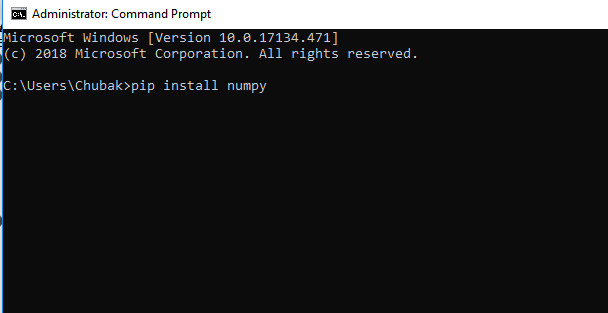
\includegraphics[scale=0.8]{pip_1}
	 	\end{center}
	 \end{enumerate}  
	 
	 
	 وقتی پکیج روی کامپیوترمان نصب شد، میتوانیم با فرمانهای زیر، در اول یا هرجای فایل اسکریپت، پکیج را \textbf{وارد}\footnote{Import} اسکریپتمان کنیم.
	 
	 
	 
	 	 	 \begin{latin}
	 	\mono{	\begin{lstlisting}[backgroundcolor = \color{lightgray}]
import numpy
from numpy import class
import numpy as math
	 		\end{lstlisting}}	 
	 	
	 \end{latin}
 
 چندین نوع وارد کردن وجود دارد. اولی، همانطور که میبینید، وارد کردن کل پکیج است. وقتی اینکار انجام شد. میتوانیم با استفاده از فرمان \lr{\mono\lstinline|numpy.method()|} اسلوبها و خواصهای مورد نظر خود را استفاده نماییم. روش دوم، وارد کردن کلاسی خاص با استفاده از فرمان \lr{\mono\lstinline|from x import y|} است. و فرمان سوم، نام پکیج مورد نظر را تغییر میدهد. 
	 
	 
	 هر پکیج راهنمای خود را دارد که در اینترنت پیدا میشود. در این کتاب، وقتی از یک پکیج نام میبریم، دیگر نمیگوییم آنرا چگونه نصب کنید. وظیفه ی خودتان است که پکیج را نصب کرده و وارد نرم افزار کنید.
	 
	 \subsection{پایان بخش پایتان}
	 
	 با پایان رسیدن بخش پایتان، لازم است یادآوری کنم که من فقط پوسته ی پایتان را خراش دادم. اگر میخواهید بیشتر بدانید، کتابهای متعددی برای اینکار وجود دارند.
	 
	 
	 
	 \section{\lr{C++}}\label{cpp}
	 زبان \lr{C++} در اوایل دهه ی هشتاد توسط دکتر بی ‌یارنه استراستروپ، مهندس دانمارکی، ابداع شد. فرق \lr{C++} با C در برنامه نویسی شیء گراست. این زبان، عوض پایتان، \textbf{کامپایل}\footnote{Compile} میشود. یعنی، توسط یک نرم افزار به نام کامپایلر که به زبان C نوشته شده، به زبان اسمبلی تبدیل میشود و سپس سیستم عامل آنرا به زبان ماشین تبدیل کرده و آنرا اجرا میکند. 
	 
	 
	 کامپایرهای زیادی برای \lr{C++} وجود دارند. دو تا از بزرگترین کامپایلرها، GCC روی لینکس و \lr{Microsoft Visual C++} روی ویندوز است. البته روی ویندوز میتوان از MinGW یا Cygwin هم استفاده کرد.
	  
	 محیط گسترش مجتمع روی ویندوز، برای \lr{C++} زیاد است. اما ما از \lr{Microsoft Visual Studio} استفاده میکنیم. پیشنهاد نمیکنم این نرم افزار را به صورت پایریت شده از بازار بخرید، بلکه، پیشنهاد میکنم نسخه ی مجانی Community آنرا از سایت مایکروسافت دانلود کرده و آنرا نصب کنید.
	 
	 \url{https://visualstudio.microsoft.com/vs/community/}
	 
	 
	  یادتان باشد هنگام نصب، \lr{Visual C++ Tools} را نصب کنید. وگرنه از منوی Tools میتوانید پکیج را نصب کنید. یکی از نیکوییهای ویژوال استودیو، \lr{NuGet Package Manager} است که به شما اجازه میدهد فایلهای \textbf{سَری}\footnote{Header} کتابخانه ها را دانلود کنید. اما ما خودمان فایلهای سَری را دانلود کرده و \textbf{اضافه}\footnote{Include} میکنیم. به معرفی \lr{C++} بپردازیم. چون خیلی از چیزها تکرار از بخش پایتان میباشد، این بخش بسیار کوتاه خواهد بود.
	  
	 برای شروع یک پروژه ی جدید از بخش \lr{File - > New Project} یک پروژه ی \lr{Windows Console Application} بسازید. 
	 
	 \begin{center}
	 	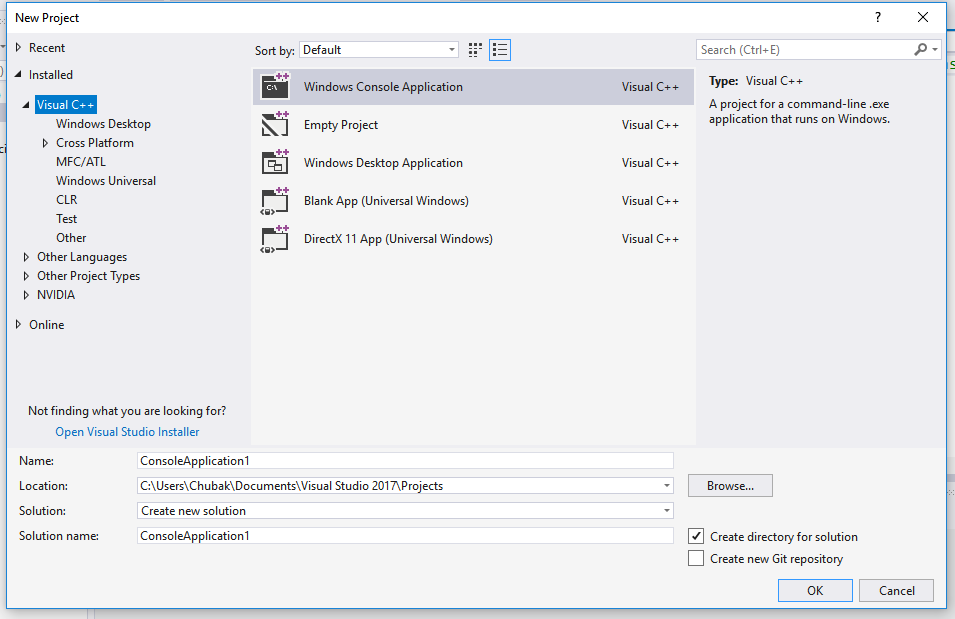
\includegraphics[scale=0.4]{VSNewProject}
	 \end{center}
	 
	 \subsection{سینتکس}\label{cppsyn}
	 
	 یک برنامه ی \lr{C++} به صورت زیر نوشته میشود:
	 
	 	 	 	 \begin{latin}
	 	\mono{	\begin{lstlisting}[backgroundcolor = \color{lightgray}]
#include "pch.h"
#include <iostream>
	 	
int main()
{
	std::cout << "Hello World!\n"; 
}
	 		\end{lstlisting}}	 
	 	
	 \end{latin}
	 
	 کلمه ی کلیدی \lr{\mono\lstinline|#include|} فایلهای سَری برنامه را تعیین میکنند. فایلهای سری، \textbf{اعلامیات}\footnote{Declaration} توابع، متغیرها، و کلاسهای برنامه هستند. \textbf{تعیینات}\footnote{Definitions} برنامه در فایلهای سورس برنامه قرار دارند. هر فایل سری با پسوند .h، یک فایل سورس با همان نام با پسوند .cpp دارد که حاوی تعیینات برنامه است. 
	 
	 تابع \lr{\mono\lstinline|main|} تابع اصلی برنامه است. اگر یک برنامه، تابع اصلی نداشته باشد، کتابخانه به حساب می آید. در \lr{C++} برخلاف پایتان نمیتوانیم یک کد را خارج از تابع به اجرا درآوریم، و تابع اصلی برای همین کار است. 
	 
	 متد \lr{\mono\lstinline|std:cout|} $ \text{(تلفظش سی-اوت میباشد)} $ یکی از اسلوبهای کتابخانه ی \textbf{STL}\footnote{\lr{Standard Template Library}} میباشد. std که با دو تا دونقطه از اسلوب سی-اوت جدا شده، \textbf{فضانام}\footnote{Namespace} اسلوب میباشد.  فضانامها مجمعه ای از اسلوبها هستند که مسمای آنان، کتابخانه شان است. std مسمای اسلوبهای کتابخانه ی STL است.
	 
	 از علامت \lr{\mono\lstinline|>>|} تعجب نکنید، این یک آپریتور بیت وایز میباشد. اما درینجا معنی "خروج" میدهد. با زدن \lr{\keys{\ctrl + F5}} خروجی نرم افزار را خواهید دید.
	 
	 \begin{center}
	 	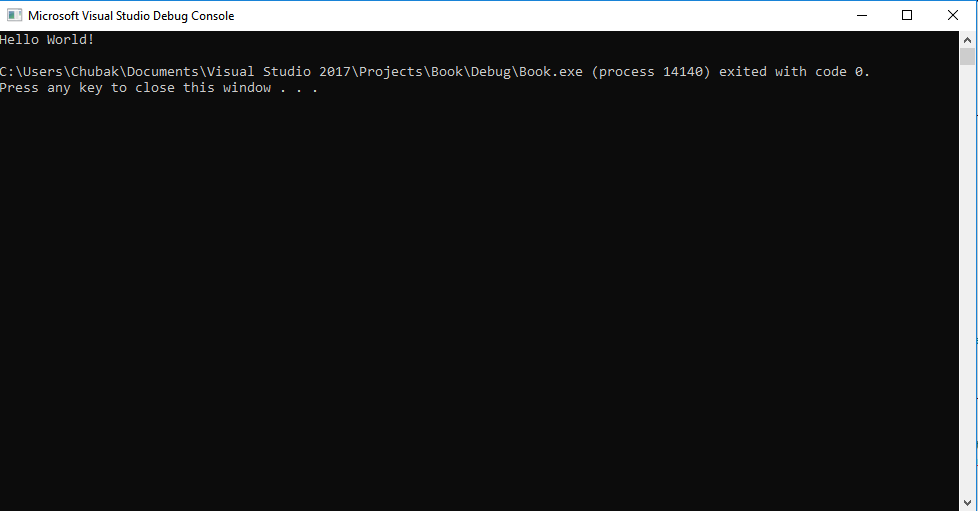
\includegraphics[scale=0.3]{HelloWorld}
	 \end{center}
	 
	 
	 تابع معکوسِ سی-اوت، \lr{\mono\lstinline|std::cin|} $ \text{(سی-این)} $ میباشد. سی-این یک متغیر را گرفته، و به از کیبورد ارزش گرفته و به آن مقداردهی میکند.
	 
	 	 	 	 	 \begin{latin}
	 	\mono{	\begin{lstlisting}[backgroundcolor = \color{lightgray}]
int main()
{
	int variable = 0;
	std::cin >> variable;
	std::cout << variable << std::endl;
}
	 		\end{lstlisting}}
 	
	 	
	 \end{latin}
	 
	 
	 کدِ بالا، توسط سی-این، یک عدد به متغیر میدهد و بعد آنرا به نمایش میگذارد. \lr{\mono\lstinline|std::endl|} که حرف آخرش L کوچک است، خط جدید ایجاد میکند.
	 همانطور که توجه کرده اید، متغیرها در \lr{C++}، نوع دارند چون \lr{C++} زبان تایپ امن است. زیر زیر چند گونه از انواع دیتا در این زبان را مشاهده میکنید.
	 	 	 	 \begin{latin}
	\mono{	\begin{lstlisting}[backgroundcolor = \color{lightgray}]
//integer
unsigned int;
signed int;

unsigned short;
signed short;

unsigned long long;
signed long long;

unsigned long;
signed long;

//decimal
float;
double;
long double;

//text
char;
wchar_t;

//rest
bool;
void;

		\end{lstlisting}}	 
	
\end{latin}
	 
	 
	 
	 تمام اعداد صحیح دو حالت دارند، signed و unsigned. همانطور که بر می آید، اگر یک عدد صحیح signed باشد، میتواند اعداد منفی نیست دریافت کند. اما اگر عدد صحیح unsigned باشد، بین 0 و مکسیمم اعداد صحیح پذیرفته شده توسط پراسسور کامپیوتر است. مکسیمم short، یک عدد بسیار کوچکتر از مکسیمم int بوده، و مکسیمم long و long long بسیار از مکسیمم int بیشترند. اما long و long long، با استفاده از \textbf{حقه های اتاق نشیمن}\footnote{\lr{Parlor Tricks}} مکسیمم بیشتری دارند. مکسیمم واقعی اعدادی که یک کامپیوتر دریافت میکند، توسط \textbf{واحد پراسسور مرکزی}\footnote{\lr{Central Processing Unit or CPU}} تعیین میشود. مثلا یک پراسسور 32 بیتی میتواند بین   -2,147,483,647 و 2,147,483,647 عدد صحیح نگه دارد که مساوی $ 2^{31} $ میباشد. یک پراسسور 64 بیتی $ 2^{63} $ مکسیمم عدد نگه میدارد. علت اینکه 31 و 63 است اینست که، یکی از بیتها برای علامت منفی یا مثبت عدد نگه داشته میشود. اما معنی 32 بیت و 64 بیت چیست؟ در بخش \ref{refpointer} خواهید خواند. در \lr{C++}، متفیر int، 32 بیتی است. اما در کتابخانه ی استاندارد، int 64 بیتی نیز یافت میشود.
	 
	 متغیرهایی که عدد اعشار میپذیرند،  سه نوعند. فلوت، که در پایتان با آن آشنا شدیم، \textbf{دابل}\footnote{Double} که \textbf{دقت}\footnote{Percision} آن دو برابر فلوت است، و دابل طولانی، که دقتش چندین برابر دابل معمولی است.
	 
	 \begin{tip}
	 	شاید برایتان سوال باشد که از فلوت استفاده کنید یا از دابل. جواب، در احتیاجات شماست. مثلا اگر $ \pi $ را حساب کنیم، و آنرا یک بار در فلوت قرار بدهیم، یکی بار در دابل، یک بار در لانگ دابل:	 		 	 	 	 \begin{latin}
	 		\mono{	\begin{lstlisting}[backgroundcolor = \color{lightgray}]
//float:
3.1415927410125732421875 
//double:
3.141592653589793115997963468544185161590576171875 
//long double:
3.1415926535897932385128089594061862044327426701784133911132812
	 			\end{lstlisting}}	 
	 		
	 	\end{latin}
	 \end{tip}
	 
	 
	 
	 \lr{\mono\lstinline|char|} و \lr{\mono\lstinline|wchar_t|} انواع کاراکتر در \lr{C++} هستند. اولی، فقط کاراکترهای \textbf{اسکی}\footnote{ASCII - کیبورد استاندارد آمریکا} دومی کاراکتر های \textbf{یونیکد}\footnote{Unicode - کاراکتر ستی که تمام کاراکترهای دنیا، حتی خط میخی پارسی، را در بر دارد.} را قبول میکند. میتوان خود کاراکتر را به این متغیر داد، یا شماره ی آن در یونیکد یا اسکی را.
	 
	 در \lr{C++} مانند پایتان، نوع استرینگ نداریم. اما در کتابخانه ی استاندارد استرینگ داریم که \lr{\mono\lstinline|std::string|} نام دارد. برای استفاده از بخش استرینگِ کتابخانه ی استاندارد مانند زیر عمل میکنیم:
	 
	 
	 
	 	 		 	 	 	 \begin{latin}
	 	\mono{	\begin{lstlisting}[backgroundcolor = \color{lightgray}]
#include <iostream>
#include <string>

int main()
{
	std::string myString = "Text";
}


	 		\end{lstlisting}}	 
	 	
	 \end{latin}
	 
	 
	 
	 
	 با تایپ بولی نیز آشنا هستید. تایپ ووید، یعنی تایپ خالی. کاربرد آن، کم است.
	 هرنوع تایپ را میشود ترکیب کرد و \textbf{ثابته}\footnote{Constant} ساخت. ثابته ها، برعکس متغیرها، هرگز تغییر نمیکنند. برای ساخت ثابته از نوع فلوت به صورت زیر عمل میکنیم:
	 
	 \begin{latin}
	 	\mono{	\begin{lstlisting}[backgroundcolor = \color{lightgray}]
const float pi = 3.1415
	 		\end{lstlisting}}	 
	 	
	 \end{latin}
	 
	 
	 \subsection{متغیرهای اشاره ای و مرجعی}\label{refpointer}
	 
	 مسلما شما تابحال وقتی خواستید فایلی را دانلود کنید، به سایز آن فایل نگاه کرده اید. مثلا 10 مگابایت، 20 گیگابایت، و یا سایز هارددیسک اکسترنال شما، مثلا 1 ترابایت. هر بایت، مختص از 8 بیت است. هر بیت، یک اینستراکشن به پراسسور است: 0 یا یک. هر بایت، یک عدد \textbf{دودویی}\footnote{Binary} است و هر بیت، یک رقم آن عدد است. اعداد دودویی یا باینری، عوض ارقام 0 تا 9، از ارقام 0 و 1 تشکیل شده اند. همچنین میتواند یک بایت را به صورت \textbf{شانزده شانزدهی}\footnote{Hexadecimal} نشان داد. ارقام شانزده شانزدهی از 0 تا 16 هستند. اما ما ارقام شانزده شانزدهی را با حروف الفبا نشان میدهیم. مثلا FF مساوی 255 است.
	 	
	 از اعداد شانزده شانزدهی بگدریم و به اعداد دودویی بپردازیم. یک کامپیوتر، اینگونه عمل میکند:
	 
	 \begin{enumerate}
	 	\item ابتدا، سیستم عامل، دستورات را به صورت 0 و 1 به رم میفرسد.
	 	\item پراسسور، بسته به \textbf{ساعت}\footnote{Clock} خود، در بازی های زمانی ثابت، این دستورات را از رم وارد\textbf{باس}\footnote{Bus} خود میکند.
	 	\item دستورات باینری وارد \textbf{دروازه های منطقی}\footnote{\lr{Logic Gates}} میشوند.
	 	\item دستورات به اطلاعات تبدیل شده، و به دستگاههای خروجی داده میشوند.
 	 \end{enumerate}
  
  اطلاعات در رَم، با یک \textbf{آدرس حافظه ای}\footnote{\lr{Memory Address}} هستند. آدرس حافظه، در پایه ی شانزده شانزدهی نوشته میشود. این آدرس حافظه ای در پراسسورهای اولیه فقط 8 بیت بود، و با گذر زمان، بیشتر شد. اکثر پراسسورهای امروزی 64 بیت آدرس حافظه دارند. اما بیشتر ازین هم میشود. مثلا پراسسور \lr{Playstation 2} 128 بیت آدرس حافظه ای دارد.
  
  در \lr{C++}، حافظه به دو بخش تقسیم میشود: \textbf{پشته}\footnote{Stack} و \textbf{هرم}\footnote{Heap}. پشته، توسط پراسسور کنترل میشود و اگر سایز آن از حدی بیشتر شود، \textbf{سرریز}\footnote{Overflow} میشود. هرم، دینامیک است و توسط کاربر کنترل میشود. متغیرها را باید دَستی از پشته به هرم برد.
  
  و اما \textbf{متغیرهای اشاره ای}\footnote{Pointers}. متغیرهای اشاره ای، متغیرهایی هستند که به آدرس حافظه ی یک متغیر دیگر اشاره دارند و اینگونه درست میشوند: 
	 
	 
	 
	 \begin{latin}
	 	\mono{	\begin{lstlisting}[backgroundcolor = \color{lightgray}]
#include "pch.h"
#include <iostream>


int main()
{
	int i = rand();
	int *ip = &i;
	std::cout << "'i' is: " << i << "; " <<
	"The memory address of it is" << ip << std::endl <<
	"And by adding * to ip we 'dereference' it like so: " << *ip;
}

	 		\end{lstlisting}}	 
	 	
	 \end{latin}
	 
	 
خروجی این نرم افزار، اینست:


	 \begin{latin}
	\mono\color{white}{	\begin{lstlisting}[backgroundcolor = \color{black}]

'i' is: 41; The memory address of it is 00CFFCB8
And by adding * to ip we 'dereference' it like so: 41
	
		
		\end{lstlisting}}	 
	
\end{latin}

	

	 بگذارید این کد را مرحله به مرحله توضیح دهم:
	 \begin{enumerate}
	 	\item  ابتدا، ما،  یک متغیر به نام i درست میکنیم و یک عدد رندوم به آن میدهیم.
	 	\item  سپس، ما یک متغیر اشاره ای به نام ip درست میکنیم. برای اینکه متغیر اشاره ای درست کنیم، از علامت \textbf{ستاره}\footnote{Asterisk} استفاده میکنیم. سپس با علامت \textbf{امپرسند}\footnote{Ampersand} آدرس i را به آن میدهیم.
	 	\item سپس به کامپایلر میگوییم که اول، متغیر را پرینت کن. بعد، ارزش متغیر اشاره ای را پرینت کن، که آدرس متغیر اصلی در حافظه است. سپس، متغیر اشاره ای را \textbf{دیریفرنس}\footnote{Dereference} کن. یعنی، ارزشی که در آدرس حافظه ای که به آن اشاره میکنی ر پرینت کن.
	 \end{enumerate}
 
 عکس زیر، گویای همه چیز است.
	 
	 
	 
	 
	 \begin{figure}[H]
	 	\centering
	 	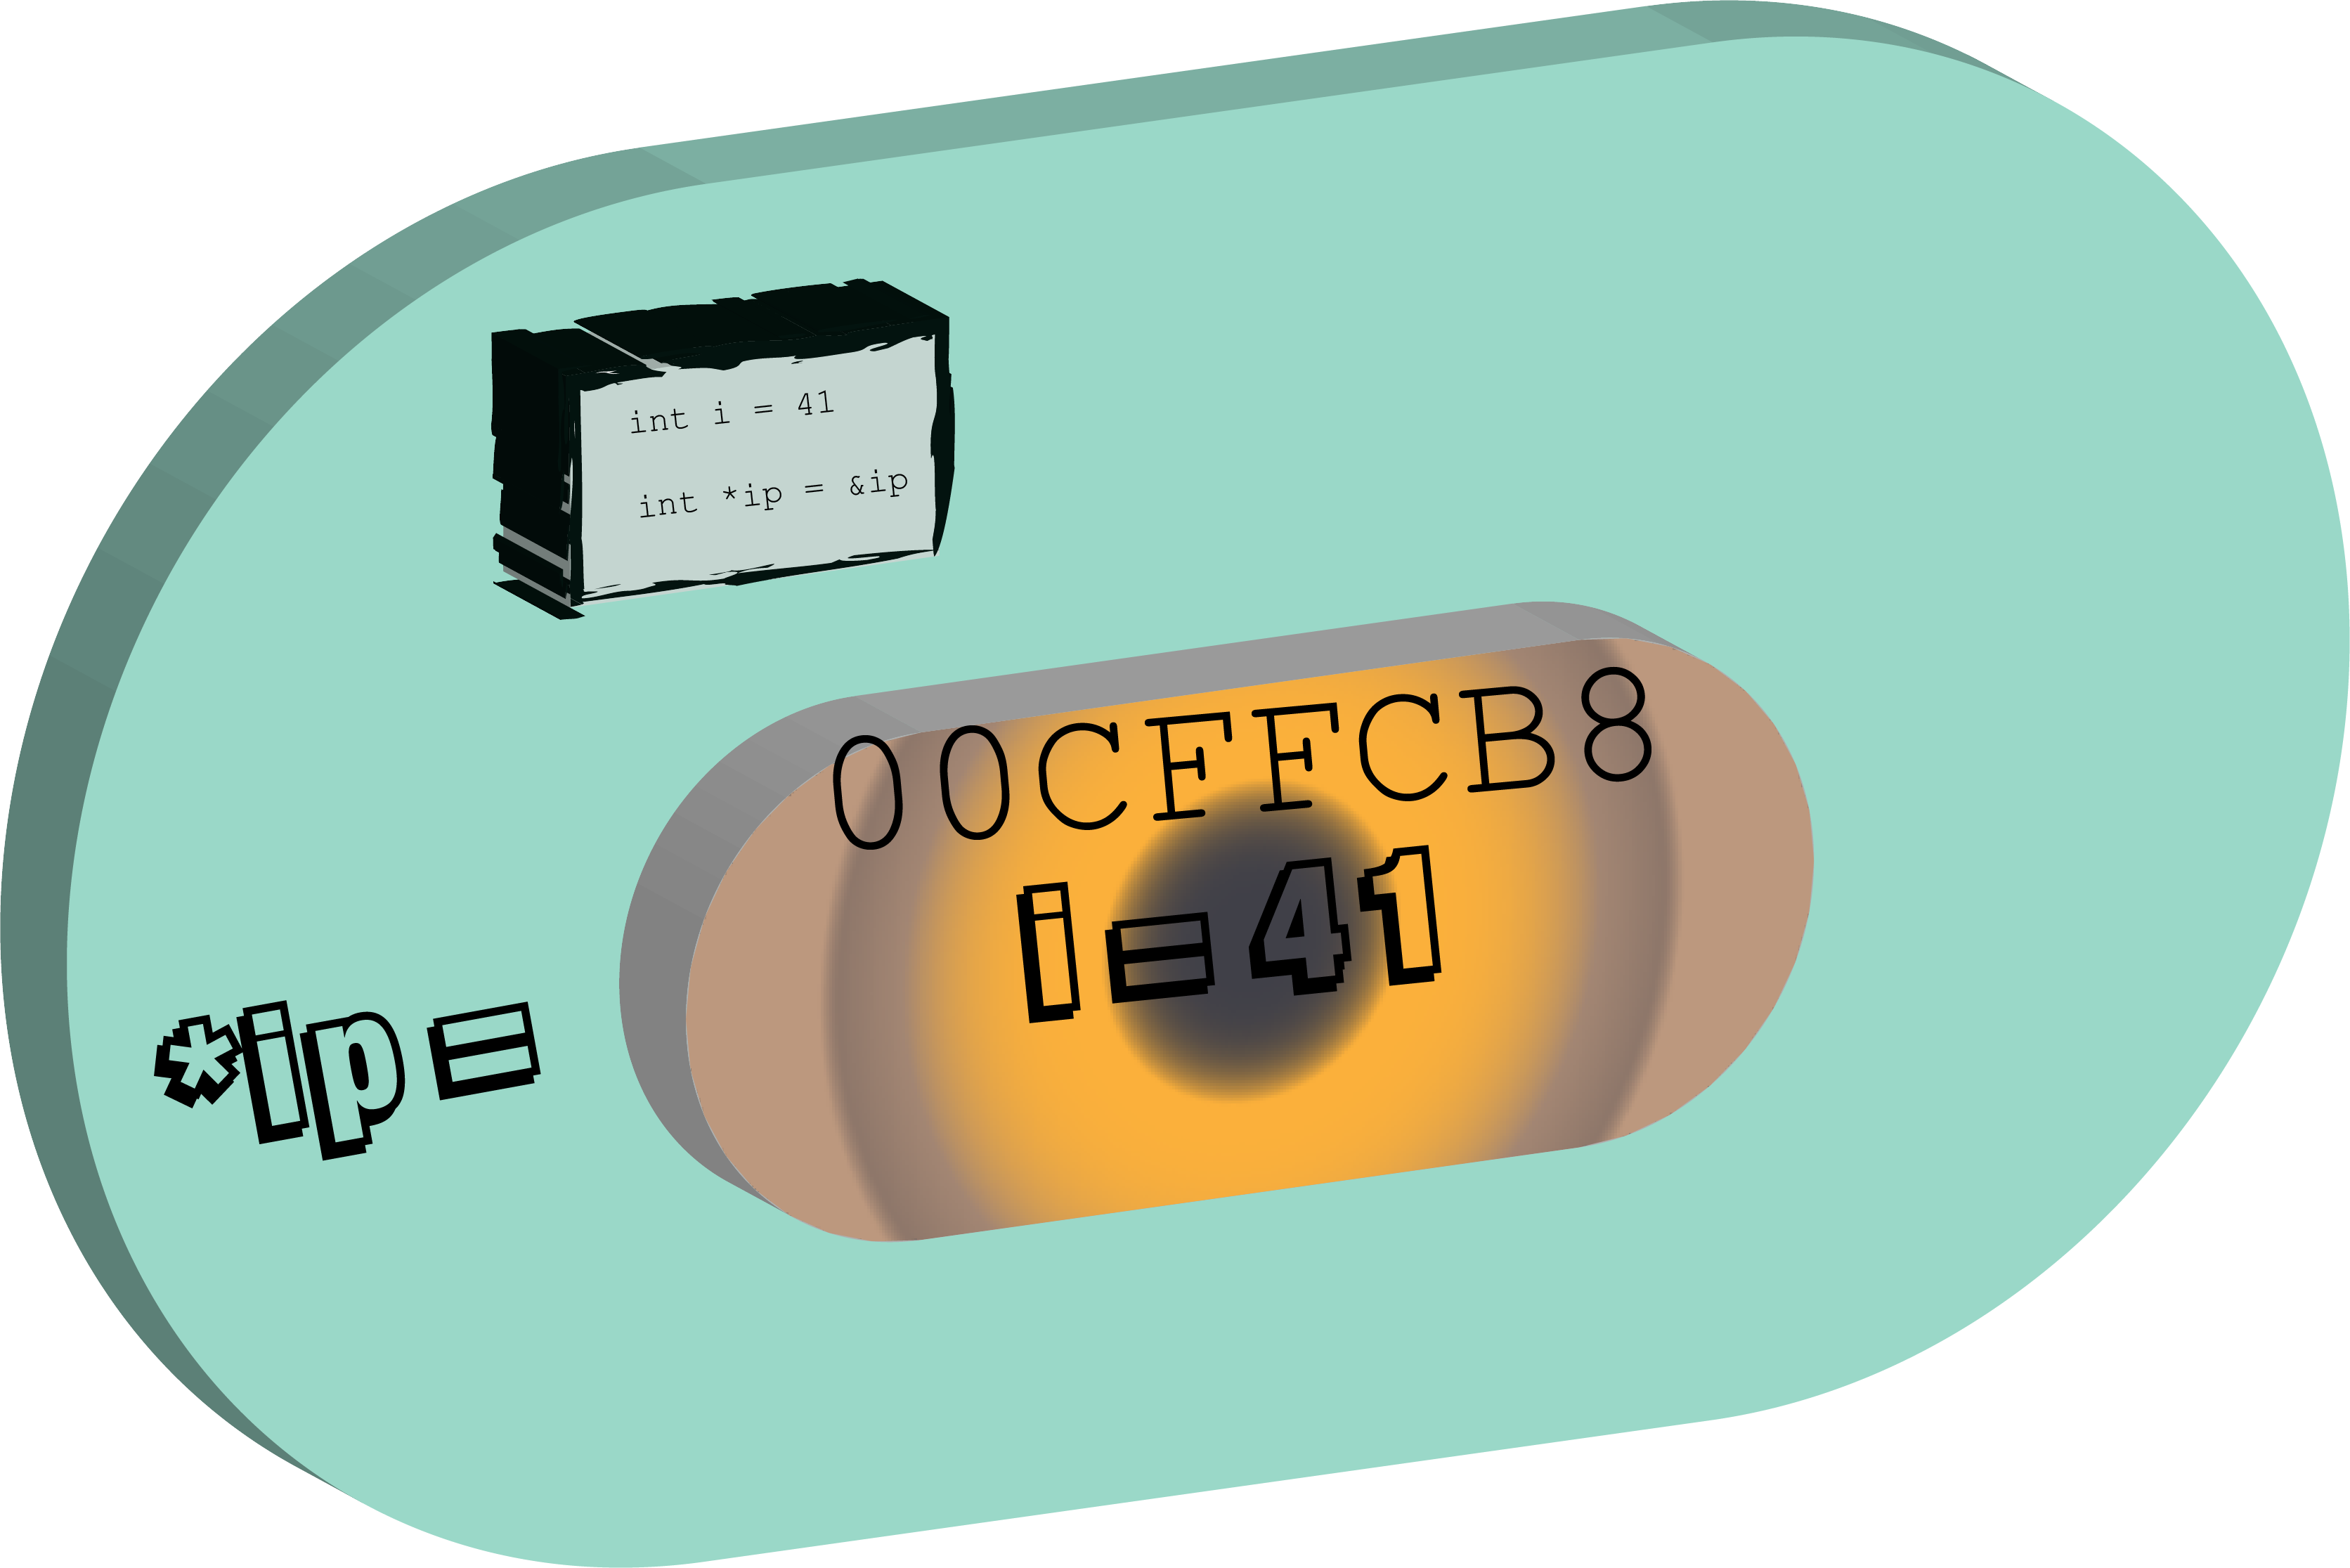
\includegraphics[scale=0.2]{MemoryAddress}
	 	\caption{آدرس حافظه و دیرفرنس کردن}
	 \end{figure}
	 
	 به \lr{\mono\lstinline|&i|} \textbf{اشاره ی مرجعی}\footnote{Reference} به i میگوییم. کلا برای اشاره مرجعی به هر متغیری، از علامت امپرسند استفاده میکنیم. در بخشهای بعد، مصرف آنرا خواهید دید.
	 
	 
	 
	 
	 
	 
	 \subsection{بیانیه های شرطی و چرخشی}\label{cppifcond}
	 
	 بیانیه های شرطی و چرخشی، در \lr{C++} مانند همتایانشان در پایتان هستند. در زیر تنها به سینتکسشان بسنده میکنیم:
	 
	 
	 
	 
	 
	 
	 	 \begin{latin}
	 	\mono{	\begin{lstlisting}[backgroundcolor = \color{lightgray}]
int i = rand();
if (i > 20)
{
	std::cout << "i is greater than 20.";
}
else if (i > 30)
{
	std::cout << "i is greater than 30.";
}
else
{
	std::cout << "i is smaller than 20 and 30.";
}
{
while (i > 0)
{
	std::{cout << i << std::endl;
	i -= 0;
}

for (int h = i; h > 0; h--)
{
	std::cout << h << std::endl;
}
	 		
	 		\end{lstlisting}}	 
	 	
	 \end{latin}
	 
while و for یک کار را انجام میدهند، فقط، اینگونه است که ابتدا \textbf{بازتکرارکننده}\footnote{Iterator} یک مقدار میگیرد، بعد شرط میگذاریم، و بعد میگوییم چقدر از مقدار کم، اضافه، ضرب یا تقسیم کن. به هرکدام ازین بیانیه هایی که در چرخش for داریم، \textbf{اصطلاح}\footnote{Expression} میگوییم. هر اصطلاح، یک بیانیه است، اما هر بیانیه ای، یک اصطلاح نیست.

\begin{tip}
	درینجا، i در \textit{اسکوپ} خارجی تابعی که کد را در آن اجرا میکنیم، قرار دارد. به اینگونه متغیرها، \textbf{جهانی}\footnote{Global} میگوییم. یک متغیر میتواند نسبت به کل کد، جهانی باشد. برای اینکار، کافیست متغیر را بیرون تابع اصلی تعیین، یا مقداردهی کنید. معمولا ثابته ها، نسبت به همه چیزِ، جهانی هستند.
\end{tip}
	 اما \lr{C++} دارای یک بیانیه ی چرخشی دیگر به نام  \textbf{do...while} هستیم:
	 
	 	 
	 \begin{latin}
	 	\mono{	\begin{lstlisting}[backgroundcolor = \color{lightgray}]
do
{
	i %= 10;
	i - 1;
}
while (i > 0)

	 		
	 		\end{lstlisting}}	 
	 	
	 \end{latin}
	 
	 
فرق do...while با while اینست که while فقط در صورتی که شرط درست باشد، یک بیانیه را اجرا میکند. اما در do...while، بیانیه ای که در برکت do قرار دارد، \textbf{یک بار} اجرا میشود تا شاید اگر لازم بود، شرط برقرار شود.


\subsection{آرایه ها، بردارها، نقشه ها}\label{cpparr}
	 
	 در \lr{C++} برای نگه داشتن چندین متغیر معمولی یا اشاره ای، چندین نوع لیست محیا شده که پایه ی همه ی آنها \textbf{آرایه}\footnote{Array} است. آرایه، یک \textit{گروه} از دیتای \textbf{هم نوع} است. اندازه ی یک آرایه، از قبل تعیین شده است و نمیتواند کاهش یا افزایش یابد. اما آرایه، جهشی بوده و میتوان اعضای آنرا توسط ایندکس داده شده، تعیین کرد.
	 
	 
	 
	 
	 	 	 
	 \begin{latin}
	 	\mono{	\begin{lstlisting}[backgroundcolor = \color{lightgray}]
int integerArray[3];
int integerArray[] = { 1, 2, 3 };
int integerArray[3] = { 0 };

std::cout << integerArray[0];

int myArray[20];
for (int i = 0; i < 20; i++)
{
	myArray[i] = rand();
}
	 		
	 		\end{lstlisting}}	 
	 	
	 \end{latin}
	 
	 
	 
	 \begin{enumerate}
	 	\item ابتدا ما یک آرایه  با 3 عضو میسازیم. این آرایه، خالی است.
	 	\item سپس ما یک آرایه با 3 عضو ساخته به و به آن اعضای 1، 2 و 3 را میدهیم.
	 	\item  سپس یک آرایه ی 3 عضوی میسازیم که همه ی اعضای آن 0 است.
	 	
	 	\item  در مرحله ی بعد، یک آرایه ی 20 عضوه ساخته، و توسط بیانیه ی چرخشی for، به هر عضو آن یک عدد تصادفی میدهیم. یادتان باشد که ایندکس اعضا از 0 شروع میشود و تا سایز منهای یک ادامه دارد.
	 \end{enumerate}
 
 اما نمیتوان به آرایه عضوی اضافه و کم کرد. پس برای اینکار از چه استفاده کنیم؟ جواب، استفاده از یک \textbf{لیست زنجیره ای}\footnote{\lr{Linked List}} به نام \textbf{بردار}\footnote{Vector} میباشد. بردار، یکی از بخشهای کتابخانه ی استاندارد است. برای استفاده از بردار به صورت زیر عمل میکنیم:
 
 
	 	 \begin{latin}
	 	\mono{	\begin{lstlisting}[backgroundcolor = \color{lightgray}]
#include "pch.h"
#include <iostream>
#include <vector>

int main()
{
	std::vector<int> myVector;

	for (int i = 0; i < 20; i++)
	{
		myVector.push_back(rand());
	}

	for (auto &i : myVector)
	{
		std::cout << i << std::endl;
	}
	return 0;
}
	 		\end{lstlisting}}	 
	 	
	 \end{latin}
	 
	 
	 \begin{enumerate}
	 	\item  ابتدا با فرمان \lr{\mono\lstinline|#include|}، فایلهای کتابخانه را وارد کدمان میکنیم.
	 	\item  سپس، یک بردار با نوع int میسازیم. 
	 	\item  بعد از آن، بردارمان را برای 20 بار یک عدد تصادفی واردش میکنیم. اسلوب \lr{\mono\lstinline|push_back()|} برای اینکار است.
	 	\item سپس با استفاده از یک چرخش forِ \textbf{برداری}\footnote{Ranged} تمام اعداد را روی صفحه پرینت میکنیم.
	 \end{enumerate}
 
 در پایتان دیدیم که اگر بخواهیم یک لیست داشته باشیم که همتا به همتاست، باید از دیکشنری استفاده کنیم. اما در \lr{C++} از یک \textbf{نقشه ی آمیزشی}\footnote{Hashmap} به نام \textbf{نقشه}\footnote{Map} استفاده میکنیم. دو نوع نقشه داریم، \textbf{ترتیبی} و \textbf{غیرترتیبی}. ما از نقشه ی غیرترتیبی استفاده میکنیم.
 	 	 \begin{latin}
 	\mono{	\begin{lstlisting}[backgroundcolor = \color{lightgray}]
#include "pch.h"
#include <iostream>
#include <map>

int main()
{
	std::map<int, char> myCharMap;
	char string[] = "Hello World!";

	for (int i = 0; i < 12; i++)
	{
		myCharMap[i] = string[i];
	}

	for (auto &i : myCharMap)
	{
		std::cout << i.first << " : " << i.second << std::endl;
	}
	
	return 0;
}
 		\end{lstlisting}}	 
 	
 \end{latin}
 
	 \begin{enumerate}
	 	\item ابتدا، فایل سری نقشه را وارد میکنیم.
	 	\item  سپس، یک نقشه میسازیم که ایندکسش int و ارزشش char باشد.
	 	\item  سپس یک آرایه ی کاراکتری میسازیم و به آن یک متن میدهیم.
	 	\item سپس یک چرخش به اندازی سایز آرایه کاراکتری میسازیم و به هر ایندکس نقشه، یک کاراکتر از آرایه را میدهیم.
	 	\item  در آخر، با استفاده از خواصهای first و second در یک for برداری، ایندکسها و ارزشها را پرینت میکنیم.
	 \end{enumerate}
	 
	 
	 
	\begin{tip}
		\lr{C++}، تاپل نیز دارد. و همچنین چندین نوع دیتای دیگر. برای اطلاعات بیشتر در مورد هر چیزی از این زبان، میتوانید از اینترنت کمک بگیرید.
	\end{tip}
	 
	 
	 \subsection{توابع در \lr{C++}}\label{cppfunc}
	 
	 توابع در \lr{C++} یک نوع برگشت دارند، و چندین پارامتر با انواع مختلف میپذیرند. تابع main یک تابع int است چون یک عدد صحیح باز میگرداند. توابع در دو مرحله ساخته میشوند، اعلامیه و تعیینیه. اکثر اوقات، اعلامیه در فایلهای سَری انجام میپذیرد و تعیینیه در فایلهای سورس. اما اعلامیه همواره لازم نیست، و میتوان بدون اعلام کردن یک تابع، آن را تعیین کرد. تعیین کردن یک تابع اینگونه صورت میپذیرد:
	 
	 
	  	 	 \begin{latin}
	 	\mono{	\begin{lstlisting}[backgroundcolor = \color{lightgray}]
int numberOfDigits(int num)
{
	std::vector<int> digits;

	do
	{
		digits.push_back(num % 10);
		num /= 10;
	} while (num > 0);

	return digits.size();

}
	 		\end{lstlisting}}	 
	 	
	 \end{latin}
	این تابع، تعداد ارقام یک عدد صحیح را باز میگرداند. 
	
	\begin{tip}
		در تابع قبلی، از یک \textbf{الگوریتم}\footnote{Algorithm} استفاده کردیم. به یک سری دستور که باهم، یک کار خاص را انجام میدهند، الگوریتم میگویند. زبان \lr{C++} دارای یک کتابخانه به نام \lr{\mono\lstinline|<algorithm>|} است که الگوریتمهای لازمه برای کار روی لیستها را به ما میدهد. در بخشهای بعد از الگوریتمهای گرافیک کامپیوتری، برنامه نویسی گرافیکی، و بازی سازی حرف خواهیم زد.
	\end{tip}
	 
	 
	 اگر نوع دیتایی که تابع باز میگرداند، با نوع دیتایی که اول تابع تعیین کرده باشید، یکی نباشد، \textbf{خطای زمان کامپایل}\footnote{\lr{Compile Time Error}} میگیرید. یکی دیگر از انواع خطا، \textbf{خطای زمان اجرا}\footnote{\lr{Run-Time Error}} میباشد. برای جلوگیری از این نوع خطای زمان اجرا، از \textbf{Try...Catch} و \textbf{throw }استفاده میکنیم. به این منوال، \textbf{کنترل استثنائات}\footnote{\lr{Exception Handling}} میگویند.
	 
	 
	 
		  	 	 \begin{latin}
		\mono{	\begin{lstlisting}[backgroundcolor = \color{lightgray}]
int division(int a, int b)
{
	if (b == 0)
	{
		throw "Division by Zero!"
	}

	return a / b;

}

int main()
{
	int a = 10;
	int b = 0;

	try
	{
		std::cout << a / b;;
	}
	catch (const std::exception& e)
	{
		std::cerr << e;
	}

}
			\end{lstlisting}}	 
		
	\end{latin} 
	 
	سی-ار یا std::cerr بخشی از کتابخانه ی استاندارد است که وظیفه ی آن نمایش استثنائات انداخته شده توسط برنامه است.
	
	\subsection{کلاسهای \lr{C++}}\label{cppclasses} 
	 
	 کلاسها، مهمترین بخش \lr{C++} هستند. اصلا این زبان از اول برای برنامه نویسی شیء گرا درست شد. یک کلاس به صورت زیر است:
	 
	 
	 
	 
	 
	 
	 
	 		  	 	 \begin{latin}
	 	\mono{	\begin{lstlisting}[backgroundcolor = \color{lightgray}]
class Ancestor
{
public:
	Ancestor() = default;
	Ancestor(int x, int y, int z) { x = x; y = y; z = z };


	int returnX() { return x };

	int doSomething() override;

private:
	int x;
	int y;
	int z;

};



class Descendent : Ancestor
{
	int doSomething() { return 2*2 };
};

	 		\end{lstlisting}}	 
	 	
	 \end{latin} 
	 
	 
	 
در بخش پایتان در مورد اسلوبها و خواصها حرف زدیم. آیا میتوانید اسلوبها و خواصهای کلاس Ancestor را پیدا کنید؟

یکی از تابعهای Ancestor با کلمه ی کلیدی override مشخص شده است. اینکار برای اینست که میخواهیم کلاسهای فرزند این کلاس، این تابع را تعیین کنند. به این کار، همانطور که در بخش پایتان گفتیم \textit{چندریختی گری} یا پولی مورفیسم میگوییم.

خیلی کم اتفاق می افتد که یک اسلوب را داخل همان کلاس تعیین کنیم. معمولا کلاسها را در فایل سری اعلام، و اسلوبهایش را در فایل سورس تعیین میکنیم. در طول کتاب به مراتب این کار را انجام خواهیم داد.


	 
	 
	 
	 \subsection{پایان بخش \lr{C++}}
	 
	من اصلا پیشنهاد نمیکنم که به این توضیحات کم قناعت کنید. حتما یک کتاب بخرید و آنرا بخوانید، و یا از منابع اینترنتی استفاد کنید. هرکار میکنید، حتما مطالعه ی زبانی خود را گسترش دهید.
	
	
	
	\section{سیستمهای کنترل نسخه}\label{revcontrol}
	 
	 \textbf{سیستمهای کنترل نسخه}\footnote{\lr{Version Control Systems}} سیستمهایی هستند که با استفاده از آنها میتوانید کدهای خود را ارگانیزه کرده و در اینترنت یا کامپیوتر خود دخیره کنید. معروفترین سیستمهای کنترل ورژن، Git و SVN هستند.
	 
	 سایت Github که بزرگترین سایت Git میباشد، میتواند یک \textbf{ریپازیتوری}\footnote{Repository} برای فایلهای متنی شما درست کند و با سیستم کنترل ورژنِ Git، فایلها را Commit و Push کند. کافیست نرم افزار دسکتاپ گیتهاب را دانلود کرده، یک ریپازیتوری بسازید، کدهای خود را در آن قرار بدهید و چند وقت یک بار Pull، Commit و Push کنید. توضیحات بیشتر را میتوانید از خود سایت بیابید. من اصلا کار بدون یک سیستم کنترل ورژن را پیشنهاد نمیکنم. من در حالی که این کتاب را مینویسم، دارم هرزگاهی تغییراتم را گردآوری کرده، و کامیت، و پوش میکنم. ریپازیتوری این کتاب را میتوانید در لینک زیر بیابید.
	 
	 \url{https://github.com/Chubek/Book}
	 
	 \section{پایان فصل برنامه نویسی}
	 خوب، فصل برنامه نویسی هم به پایان رسید. همانطور که بارها در طول فصل گفتم، این به مثابه ی این نیست که برنامه نویسی را \textit{یاد} گرفته باشید. یادگرفتن برنامه نویسی سالها وقت میبرد. اما تا وقت هست، وقت تمرین هست. تمرین کنید تا یاد بگیرید. و در حین تمرین، یاد خواهید گرفت. هرگز ناامید نشوید چون هربار که زمین بخورید، دوبار بلند خواهید شد. کدهای خود را به اشتراک گذاشته و از سوال پرسیدن نترسید. 
	 
	میتوانید با استفاده از سایتهایی مثل Code Wars و Leetcode به چالشهای برنامه نویسی دست پیدا کنید تا برنامه نویسیتان قویتر شود.
	 
	 
	 
	 \chapter{مفهومات پایه ی گرافیک}\label{graphicsbasis}
	 
	 
	 \section{مانیتورهای کامپیوتر}\label{displays}

امروزه در بازار، چندین نوع مانیتور وجود دارد. LCD، OLED، LED، و همه ی آنها دارای پنلهای مختلفی هستند. اما همه ی اینها \textbf{واژه های باب روز}\footnote{Buzzwords} هستند. مثلا اپل، برای مانیتورهای خود از کلمه ی Retina استفاده میکند. در عین حال، تمام مانیتورهای امروزی، و مانیتورهای قدیمی، از یک تکنولوژی استفاده میکنند و آن تکنولوِژی \textbf{صفحه شطرنج}\footnote{Raster} است. اما صفحه شطرنج چیست؟ بگذارید ابتدا تکنولوژی مانیتورهای قدیمی و جدید را بررسی کنیم.

\subsection{مانیتورهای اشعه ی کاتدی}\label{crt}
مانیتورهای \textbf{اشعه کاتدی}\footnote{\lr{Cathode Ray Tube}} با تلوزیونهای اشعه کاتدی فرقی ندارند. تنها فرقشان درینست که، \textbf{آسیلیتور}\footnote{Ocilator} مانیتور، از \textbf{آرایه ی ویدئوگرافیکی}\footnote{VGA} دستور میگیرد، اما آسیلیتور تلوزیونهای اشعه کاتدی، از امواج الکترومغناطیس دستور میگیرند. 


\begin{tip}
	مانیتورهای جدید، از \textbf{رابط دیجیتالی ویدئو}\footnote{DVI} و \textbf{رابط چندرسانه ای با تعیین بالا}\footnote{HDMI} عوض آرایه ی ویدئوگرافیکی استفاده میکنند.
\end{tip}


همانطور که در دبیرستان آموختیم، یک اتم دارای چندین الکترون است که بار منفی دارند. با گرفتن یک الکترون از یک اتم، یک \textbf{یون }\footnote{Ion} مثبت و با اضافه کردن یک الکترون به اتم، یک یون منفی درست میکنیم. مثلا \ce{H} اتم هیدروژن، که یک الکترون بیشتر ندارد، با دارا شدن دو الکترون تبدیل به \ce{H-} و با یونیزه شدن مثبت، تبدیل به \ce{H+} میشود. به یون منفی \textbf{آنیون}\footnote{Anion} و به یون مثبت، \textbf{کاتیون}\footnote{Cation} میگویند.

به ماده ای که یک سر آن رسانا و سر دیگر آن نارسانا، نیمه رسانا، یا \textbf{خلاء}\footnote{Vacuum} است، \textbf{الکترود}\footnote{Electrode} میگویند. یک مدار الکتریکی یا الکترونیکی، معمولا از جفتهای الکترود به نام \textbf{آند}\footnote{Anode} و \textbf{کاتد}\footnote{Cathode} استفاده میکند. کاتیونها به سمت آند، و آنیونها به سمت آنود حرکت مینکند.
	 
	 در یک مانیتور اشعه کاتدی، از یک کاتد، سه \textbf{تفنگ الکترونی}\footnote{\lr{Electron Gun}} که هرکدام مسئول یک رنگ قرمز ، سبز و آبی هستند، الکترونها را به صورت نور به سمت یک آند و سپس یک پوشش نیمه رسانا شلیک میکنند و پس نور پس از گذشت از یک \textbf{ماسک سایه}\footnote{Shadow Mask}، به یک صفحه ی پوشیده از \textbf{فسفر}\footnote{Phosphorus} \ce{Ph} میرسند و بر اساس دستورات آرایه ی ویدئوگرافیکی، تصویر صفحه شطرنجی را تشکیل میدهند.
	 
	 
	 
	 \begin{figure}[H]
	 	\centering
	 	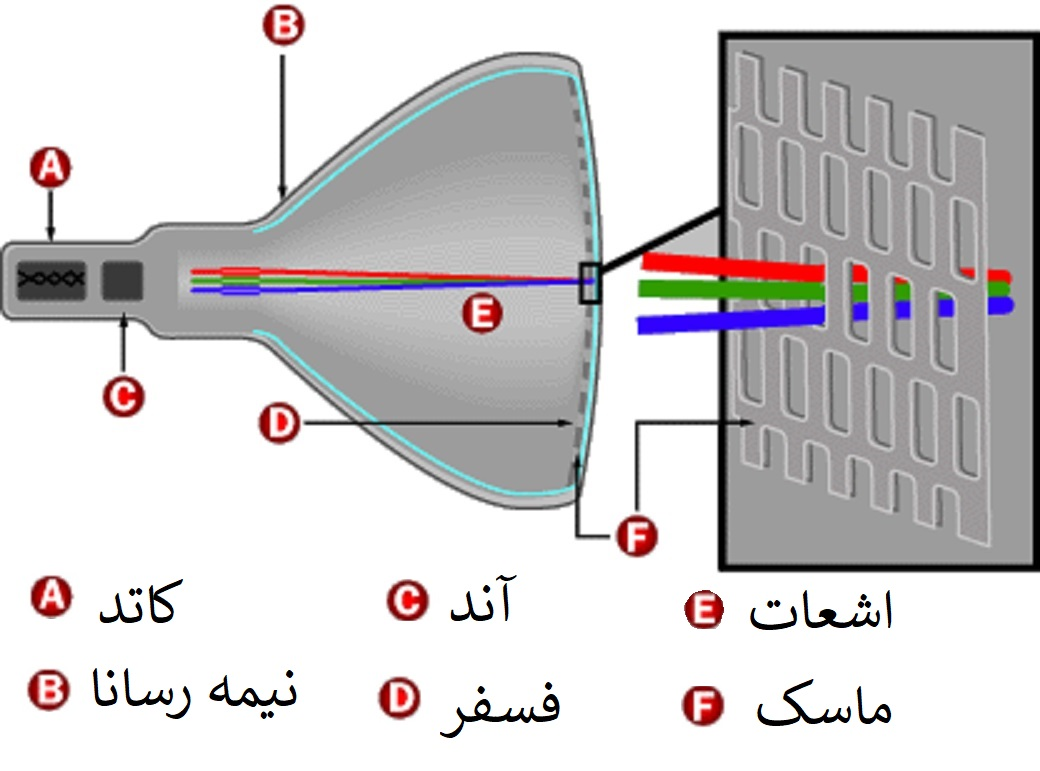
\includegraphics[scale=0.5]{CRT}
	 	\caption{مکانیزتم سی آر تی}
	 \end{figure}
	 
	 
	 \begin{tip}
	 	شاید برایتان سوال باشد که الکترون که یک \textbf{ذره}\footnote{Particle} است، چگونه تبدیل به نور میشود؟ وقتی جسم داغ میشود بعضی از الکترونها به مدار بالاتر میجهند که در حقیقت جایشان آنجا نیست و لذا ناپایدارند . موقعی که این الکترون تحریک شده دوباره به مدار خود برمیگردد یک \textbf{فوتون}\footnote{Photon} نور آزاد می شود .
	 \end{tip}
	 
	 \begin{tip}
	 	در قدیم، مانیتورهای \textbf{تک رنگه}\footnote{Monochrome}، فقط رنگ سبز را نمایش میدادند چون رنگ اصلی \ce{Ph} سبز است
	 \end{tip}
	 
	 
	 در بخش \ref{raster} به بررسی اینکه آرایه ی ویدئوگرافیکی، چگونه صفحه ی مانیتور را دستکاری میکند، حرف خواهیم زد. اما قبل از آن، به بررسی مانیتورهای \textbf{کریستال مایع}\footnote{LCD} بپردازیم.
	 
	 \subsection{مانیتورهای کریستال مایع}\label{lcd}
	 
	 مانیتورهای کریستال مایع در قدیم فقط روی  ماشین حسابها و ساعتهای دیجیتال یافت میشدند چون فقط میتوانستند یک آرایه ی هشت عضوه ی نشان دهند که با آن فقط میشد اعداد و به صورت محدود، چند حروف الفبا نشان داد. به این نمایشگر \textbf{ماژول کریستال مایع}\footnote{\lr{LCD Module}} گفته میشود، و هنوز کاربرد دارد. برای یاد گرفتن اینکه یک مانیتور کریستال مایع چگونه کار میکند، باید بفهمیم یک ماژول کریستال مایع چگونه کار میکند.
	 
	 \begin{figure}[H]
	 	\centering
	 	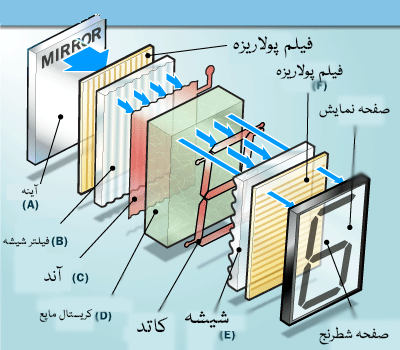
\includegraphics[scale=0.7]{LCD}
	 	\caption{چگونگی کارکرد ماژول کریستال مایع}
	 \end{figure}
	 
	 همانطور که میبینید، خود کریستال مایع بین یک آند و یک کاتد قرار دارد که شکل آند، مانند شکل \lr{\lcd 8} میباشد. بسته به دستورات باینری، این شکل تبدیل به \lr{\lcd 0, 1, 2, 3, 4, 5, 6, 7, 8, 9} میشوند. ماشین حسابهای قدیمی \textit{تگزاس اینسترامنتس}، دارای 8 ماژول کریستال مایع بودند. 
	
	
	توجه دارید که نور، یک بار قبل از بازتاب، و یک بار قبل از خروج، \textbf{پولاریزه}\footnote{Polarize} میشود. در دو عکس زیر، اثر فیلتر پولاریزه ی دایره ای را روی یک دوربین DSLR خواهید دید. عکاس هردو عکس خودم هستم. \footnote{من عاشق عکاسی هستم و یک دوربین \lr{T3i} کنن نیز دارم. میخواهم روزی از دوربینم برای ساخت تکسچر استفاده کنم.}
	
	\begin{figure}[H]
		\centering
		\includegraphics[scale=0.5]{Polar_Without}
		\caption{یک عکس گرفته شده \textbf{بدون} فیلتر پولاریزه}
		\includegraphics[scale=0.5]{Polar_With}
		\caption{یک عکس گرفته شده \textbf{با} فیلتر پولاریزه }
	\end{figure}



مانیتورهای کریستال مایع امروزی نیز مانند همین عمل میکنند، اما آند آنها، یک الکترود \textbf{ایندیم--قلع-اکسید}\footnote{\lr{Indium Tin Oxide}} است که به صورت \ce{In2O5Sn} نمایش داده میشود. این آند، میتواند رنگهای مخلتفی به خود بگیرد.  آرایه ی ویدئوگرافیکی، 256 رنگ قرمز، 256 رنگ سبز، و 256 رنگ آبی به این آند میدهد و این آند، با ترکیب آنها، $ 256^3 = 16777216 $ رنگ نمایش دهد. هررنگ همچنین دارای شدت خود است که در مورد ان صحبت خواهیم کرد. 

کنسول دستی \textbf{\lr{Game and Watch}} شرکت نینتندو از اولین کنسولهای دستی ای بود که از یک مانیتور کریستال مایع استفاده میکرد. اولین کنسول دستی ای که از مانیتور کریستال مایعی استفاده میکرد که از پشت آینه، نور میتاباند، \textbf{PSP} سونی بود. امروزه مانیتورهای کریستال مایع همه از پشت نور میتابانند. مانیتورهای LED و پلاسما هم مکانیسمی شبیه به همین دارند. اما ما، بحثمان سخت افزار نیست، بلکه بحثمان تصویری است که روی صفحه ی مانیتور نقش میبندد. مانیتورهای کریستال مدرن همه \textbf{صفحه شطرنجی} اند، یا به عبارتی، Raster. بگذارید در بخش بعد، کامل توضیح بدهم.


	 
	 \section{ صفحه ی شطرنجی و المان تصویری (پیکسل)}\label{raster}
	 وقتی من نوجوان بودم، سالها قبل ازینکه مردم با دوربینهای موبایل خود شروع به سلفی گرفتن کنند، دوربینهای دیجیتال تازه وارد بازار شده بودند. برندهای متفاوت، باعث رقابتی سخت بین سازندگان دوربین شده بود تا به مردم بباورانند که کیفیت دوربین آنها، از بقیه بهتر است. اگر کیفیت لنز، کُدک فایلها، قابلیت ضبط ویدئو، کوچک بودن دوربین، و قیمت آن، پیش غذای رقابت دوربینها بود، \textbf{مگاپیکسل}\footnote{\lr{Mega Pixel}} شیرینی خامه ای بعد از غذا بود. 
	 
	 «سلام آقا، یک دوربین میخواستم... چی دارید؟»
	 
	 «مینولتا بدون آینه، قابلیت ذخیره ی تصاویر به صورت خام، لنز قابل تعویض، قابلیت تغییر \textbf{بالانس سفیدی}\footnote{White Balance} --- ایزو تا 3200، مود منوال...»
	 
	«حاجی، اینا رو بیخیال، \textit{مگاپیکسلش چنده}؟»
	 
	 
	 و اینگونه بود که، بر اساس گفته های ریچارد داوکینز، مگاپیکسل، یک \textbf{میم}\footnote{Meme} شد.اما پیکسل چیست؟
	 
	 پیکسل کلمه ای قدیمی است که از زمان تلوزیونهای سیاه و سفید وجود داشته، و \lr{\textbf{Pic}ture \textbf{El}ement} یا \textit{المان تصویری} معنی میدهد. هر صفحه یا زیرصفحه، دارای طول$ \times $عرض پیکسل است.
	 
	  
	  \begin{figure}[H]
	  	\centering
	  	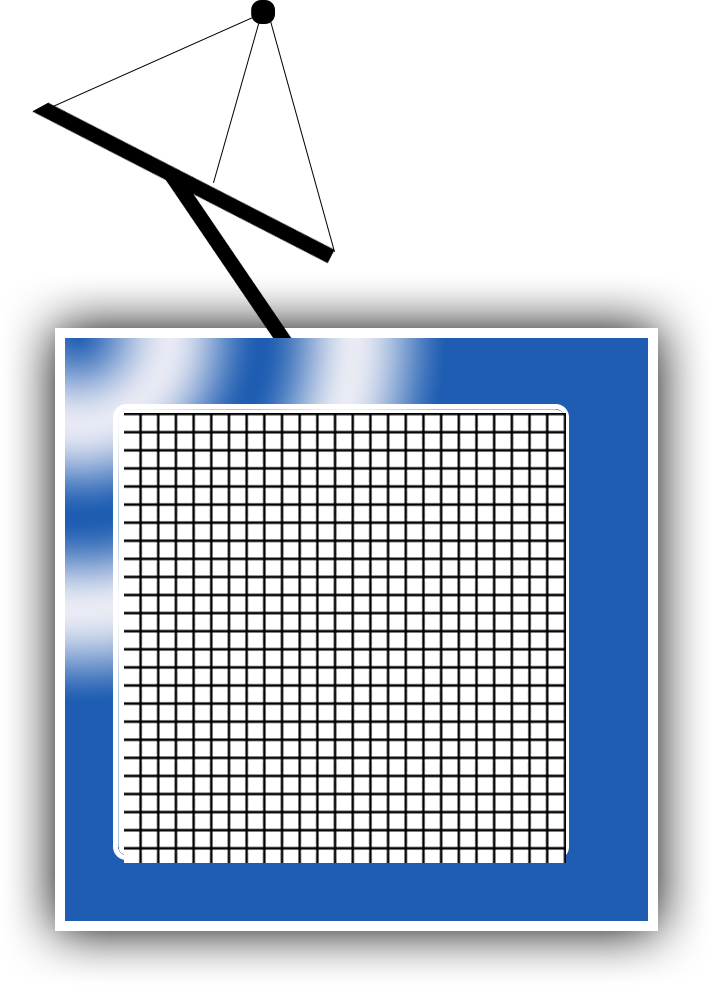
\includegraphics[scale=0.4]{TV}
	  	\caption{هر صفحه یا زیرصفحه طول $ \times $ عرض پیکسل دارد. به این مجموعه پیکسل، رستر میگویند.}
	  \end{figure}


اما صفحه ی شطرنجی یا رستر چیست؟ \textbf{به مجموعه پیکسلهای یک صفحه یا زیرصفحه، که توسط اسکن رستر یا رسترایزیشن درست شده، صفحه ی شطرنجی یا رستر میگویند}. ما ازین ببعد از کلمه ی رَستر استفاده خواهیم کرد.



 تلوزیونهای قدیمی، تقریبا در هر 100 میلی ثانیه، که به آن \textbf{آهنگ تازه سازی}\footnote{\lr{Refresh Rate}} میگویند، امواج الکترومغناطیسی که توسط \textbf{آنتن}\footnote{Aerial} دریافت میشود را تبدیل به پیکسل میگرد. تلوزیونهای قدیمی در صفحه ی خود 307200 پیکسل داشتند. 680 پیکسل افقی و 480 پیکسل عمودی. و پیکسل آنها مانند پیکسل اکثر صفحه های مدرن، مربع نبود بلکه 10:11 \textbf{نسبت }\footnote{\lr{Aspect Ratio}} داشت. این پیکسلها به صورت \textit{زیگزاگی} پر میشدند. به این امر، \textbf{اسکن رستری}\footnote{\lr{Raster Scan}} میگفتند.
 
 
	 \begin{figure}[H]
	 	\centering
	 	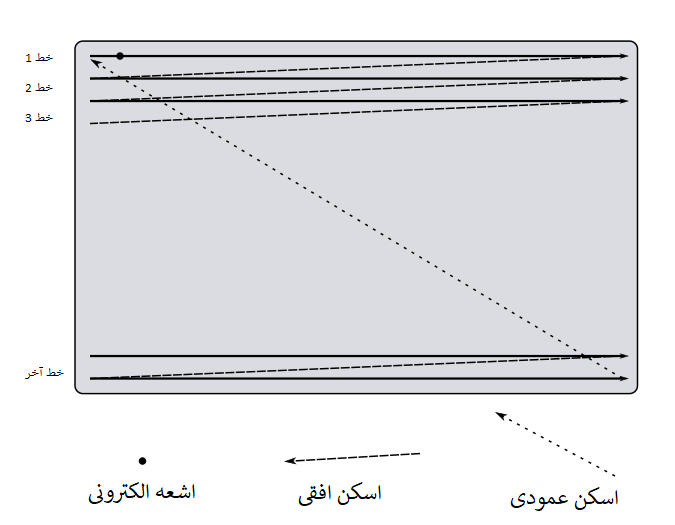
\includegraphics[scale=0.6]{RasterScan}
	 \end{figure}
	 
	 
	 اسکنرهای مدرن از همین تکنیک برای \textbf{رستر سازی}\footnote{Rasterization} دیتای خامی که اسکن میشوند، استفاده میکند. اما رسترسازی چیست؟ در بخش بعد در مورد آن صحبت میکنیم.
	 
	 \section{رسترسازی}\label{rasterize}
	 
	 
	 گفتیم که، به آرایه ای از پیکسلها، که تعداد آنها، اندازی طول تصویر ضربدر اندازی عرض تصویر است، رستر میگوییم. و همچنین گفتیم این پیکسها، به صورت زیگزاگی، در بازه زمانی خاص که همانطور که گفته شده به آن آهنگ تازه سازی میگویند، بازسازی میشوند. آهنگ تازه سازی یک \textbf{فرکانس}\footnote{Frequency} است. فرکانس، تعداد کارهای انجام شده در یک بازه است. واحد فرکانس، \textbf{هرتز}\footnote{Hrtz} میباشد. مانیتورهای اشعه کاتدی ای هستند که آهنگ تازه سازی شان 120 مگاهرتز است. اما آهنگ تازه سازی اکثر تلوزیونها و مانیتورهای کریستال مایع امروزی، 60 مگاهرتز میباشد.
	 
	 پس 60 بار در هر ثانیه، اسکن رستری صورت میپذیرد. اما برای اینکه اسکن رستری صورت بپذیرد، تمام اطلاعات تصویری داده شده به مانیتور، باید رستری باشد. چون مانیتورها همه رستری هستند و نمیوانند تصویری که رستر نیست را، نمایش دهند. به پروسه ی تبدیل تصاویری که با فرمول دو بعدی یا سه بعدی در نرم افزارهای مختلف به دست آمده اند، \textbf{رسترسازی} میگویند. به نرم افزاری که فرمولهای برداری در $ \mathbf{R^2} $ را در محیط دو بعدی، تبدیل به رستر کند، \textbf{رسترایزر}\footnote{Rasterizer} و به نرم افزاری که اشکال سه بعدی را تبدیل به رستر میکند، \textbf{رندرر}\footnote{Renderer} میگویند. یک رندرر، یک \textbf{خط لوله ی گرافیکی}\footnote{\lr{Graphics Pipeline}} میباشد که رسترایزر، جزئی از آن میباشد. در بخش \ref{api} در مورد این خط لوله بیشتر خواهید خواند.
	 
	 مثلا، نرم افزار \lr{Adobe Illustrator}، یا آلتیرنیتو مجانی آن، \textbf{\lr{Ink Escape}} --- فرمولهایی که در بخشهای بعدی بررسی خواهیم کرد، مانند الگوریتمهای به دست آوردن خط در فضای دو بعدی را، تند تند تبدیل به مجموعه ای از پیکسل کرده، و در صفحه نمایش میدهد.
	 
	 '
	 
\begin{figure}[H]
	\centering
	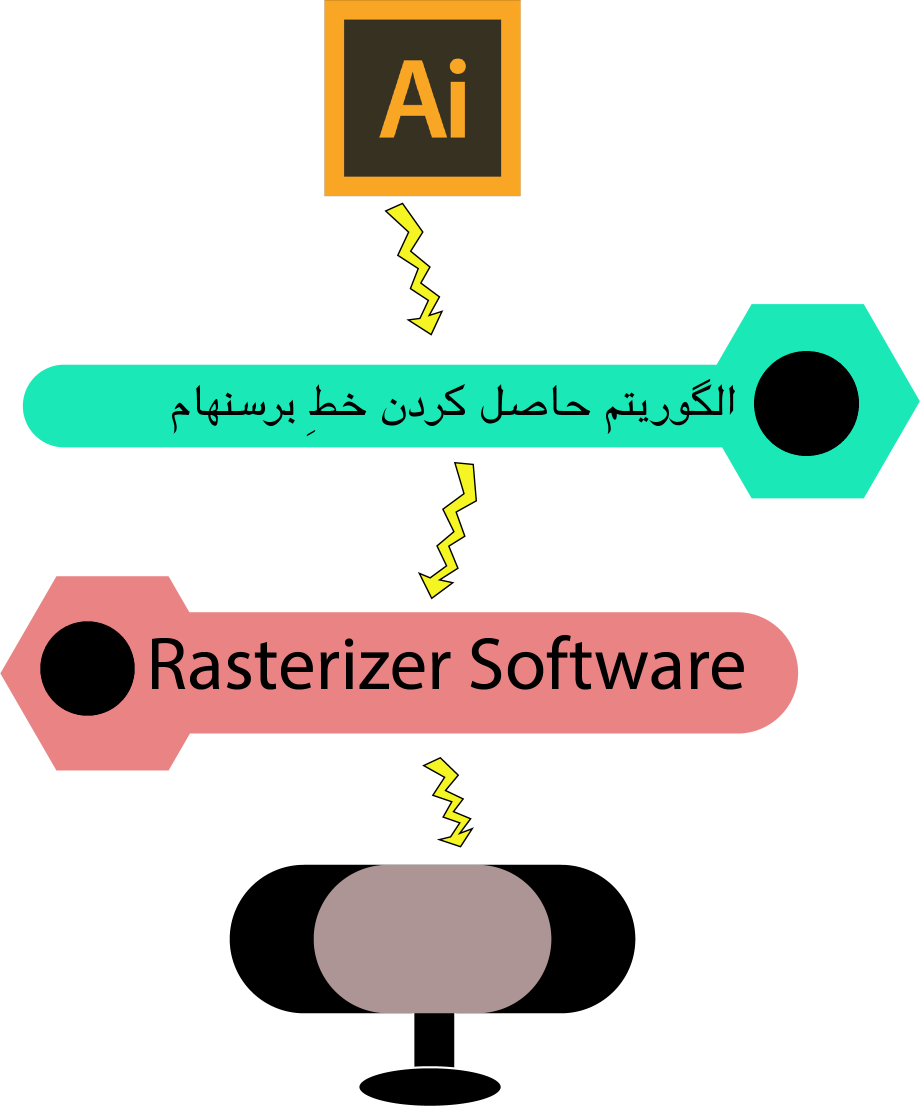
\includegraphics[scale=1]{Rasterizer}
	\caption{رسترایز آدوبی ایلوستریتر}
\end{figure}
	 
	 
	 
	 
	 اما میتوان سرنوشت یک پیکسل را مستقیما به دست گرفت. برای اینکار کافیست که از یک ادیتور رستر مانند \textbf{\lr{Adobe Photoshop}} یا \textbf{GIMP} استفاده کرد. این گونه نرم افزارها، روی هر پیکسل عکس یا تصویری که خودمان درست کرده ایم، تاثیر میگذارند. در ویدئوهایی که همراه کتاب عرضه شده اند، من به شما یاد میدهم تا با استفاده از اداره کردن پیکسلهای یک تصویر، یک \textbf{پیکسل آرت}\footnote{\lr{Pixel Art}} برای بازیهای خود بسازید.	 
	 
	 
	 شاید برایتان سوال باشد که رسترایزر، از کجا میفهمد رنگ پیکسل چیست؟ یا اینکه موقعیتش کجاست؟ در بخش بعدی درین مورد صحبت خواهیم کرد.
	 
	 
	 
	 
	 
\section{سایه زنهای ترکشی}\label{frag}

	 
	 
	 کامپیوترهای امروزی همگی از کامپیوترهای \textbf{IBM/2} نشئت میگیرند. و اینگونه کامپیوترها، در اواسط دهه ی 90، صاحب \textbf{پراسسور گرافیکی}\footnote{GPU} شدند. قبل از آن گرافیک در پراسسور مرکزی سیر روند اجرایی خود را طی میکرد. 
	 
	 
	 یک پراسسور گرافیکی، دارای چندصد \textbf{هسته}\footnote{Core} بوده که هرکدامشان چندده \textbf{رشته نخ}\footnote{Thread} کد دارند. اینگونه، پراسسور گرافیکی هزاران برنامه را در یک آن اجرا میکند.
	 
	 به این برنامه هایی که در هسته های پراسسور گرافیکی اجرا میشوند، \textbf{سایه زن}\footnote{Shader} یا شِیدر میگویند. 
	 
	 
	 
	 \begin{figure}[H]
	 	\centering
	 	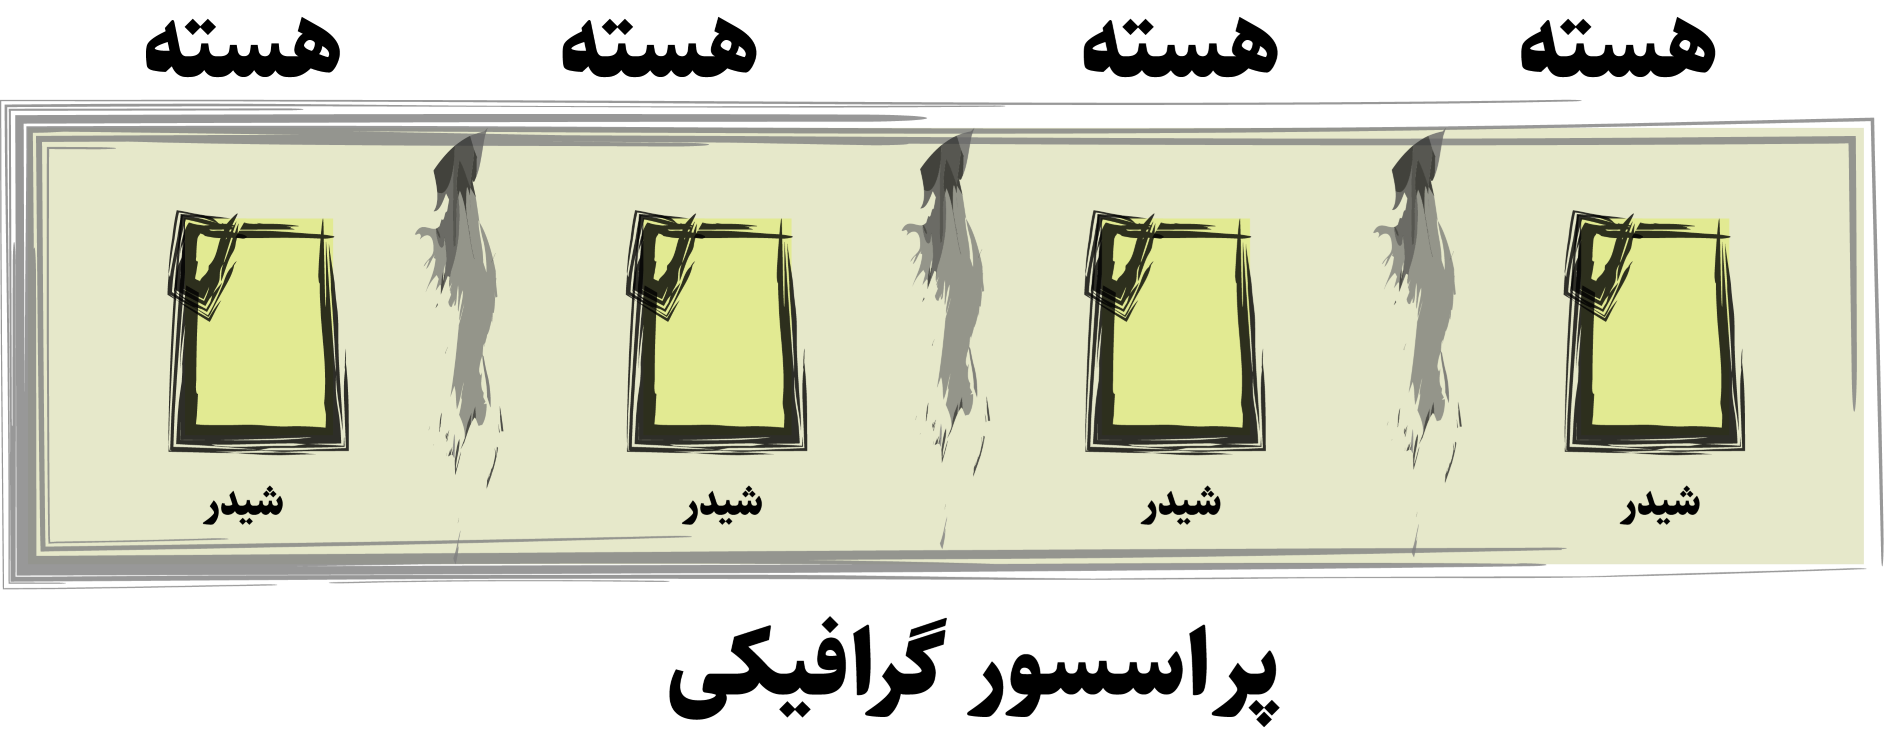
\includegraphics[scale=1]{Shaders}
	 	\caption{تمثیل شیدرها}
	 \end{figure}
	 
	 
	 چندین نوع سایه زن داریم. به سایه زنی که وظیفه اش، نگاه داشتن رنگ، موقعیت، \textbf{بیلبورد}\footnote{Billboard}، پنجره و... میباشد، سایه زن \textbf{ترکشی}\footnote{\lr{Fragment Shader}} میگوییم. در مورد سایه زن های ترکشی در طول کتاب صحبت خواهیم کرد. هر \textbf{رابط گرافیکی}\footnote{\lr{Graphics API}} مانند \textbf{دایرکت تری دی}\footnote{Direct 3D} و \textbf{اوپن جی ال}\footnote{OpenGL} زبان خود را برای سایه زنی دارد. زبان سایه زنی اوپن جی ال، GLSL نام دارد که با آن آشنا خواهیم شد. ما، ابتدا با استفاده از کتابخانه ی \textbf{پراسسینگ}\footnote{Processing} سایه زنها را اجرا، و سپس از مورد رابط گرافیکی اوپن جی ال یاد خواهیم گرفت. اینگونه، آماده خواهیم بود تا سایه زنهای \textbf{نقطه ای}\footnote{\lr{Vertex Shaders}} و سایه زنهای \textbf{هندسی}\footnote{\lr{Geometry Shaders}} را که برای ساخت اشکال سه بعدی لازمند، به راحتی یاد بگیریم.
	 
	 \section{رابطهای گرافیکی}\label{api}	 
	  
	  
	  برای هرکار گرافیکی ای در کامپیوتر که به پراسسور گرافیکی مرتبط است، احتیاج به یک \textbf{رابط برنامه نویسی کاربردی}\footnote{\lr{Application Programming Interface}} مخصوص گرافیک داریم. رابط نرم افزاری مجموعه ای از \textbf{روتینها}\footnote{Routines}، \textbf{ساختمانهای داده}\footnote{\lr{Data Structures}} و کلا، ابزاریست که مسهل برنامه نویسی هستند. گاهی اوقات، این مسهلیات فقط در حد اعلامیه هستند، اما گاها تعیینیات آنها نیز به صورت یک \textbf{کتابخانه ی دینامیک}\footnote{\lr{Dynamic Library}} که همگی شما به صورت فایلهای .DLL با آنها آشنایی دارید، عرضه میشوند. بعضی از روابط نرم افزاری \textbf{پایین دست}\footnote{Low-level} بوده، یعنی مستقیما با سخت افزار ارتباط برقرار میکنند، و بعضی از آنها \textbf{بالادست}\footnote{High-level} بوده --- یعنی با سیستم عامل ارتباط برقرار میکنند. 
	  
	  
	 دو رابط گرافیکی دایرکت تری دی و  اوپن جی ال روابط گرافیکی پایین دست بود که اولی توسط مایکروسافت، و دومی توسط گروه \textbf{Kronos} کنترل میشوند. در حالی که این کتاب نوشته میشود دایرکت تری دی 12 روی ویندوز 10 بیرون آمد، اوپن جی ال 0.6.4 به سر میبرد. دایرکت تری دی را خود مایکروسافت، تعیین کرده و میتوانید فایلهای دینامیک آنرا در پوشه ی \textbf{\lr{Windows\textbackslash System32}} بیابید. و اما اوپن جی ال، توسط هر سازنده ی کارت گرافیک، مثلا nVidia، Intel، AMD تعیین میشود و همراه درایور کارت گرافیک عرضه میشود.
	 
	 \begin{tip}
	 	همانطور که خواهیم آموخت، تمام کتابخانه های دینامیک ویندوز در پوشه ی \lr{System32}  قرار دارد. \textbf{اما} میتوان در متغیرهای محیطی، پوشه ای که کتابخانه در آن قرار دارد را اضافه ی متغیر Path کرده و اینگونه دیگر لازم نیست آنرا در \lr{System32} کپی کنید.
	 \end{tip} 
	 
	 
	 
	 اوپن جی ال برای نمایش اشکال سه بعدی روی صفحه از یا همانطور که گفتیم، \textbf{رندر} کردن آنها از خط لوله ی گرافیکی ای استفاده میکند که در زیر میبینید:
	 
	 
	 
	 \begin{figure}[H]
	 	\centering
	 	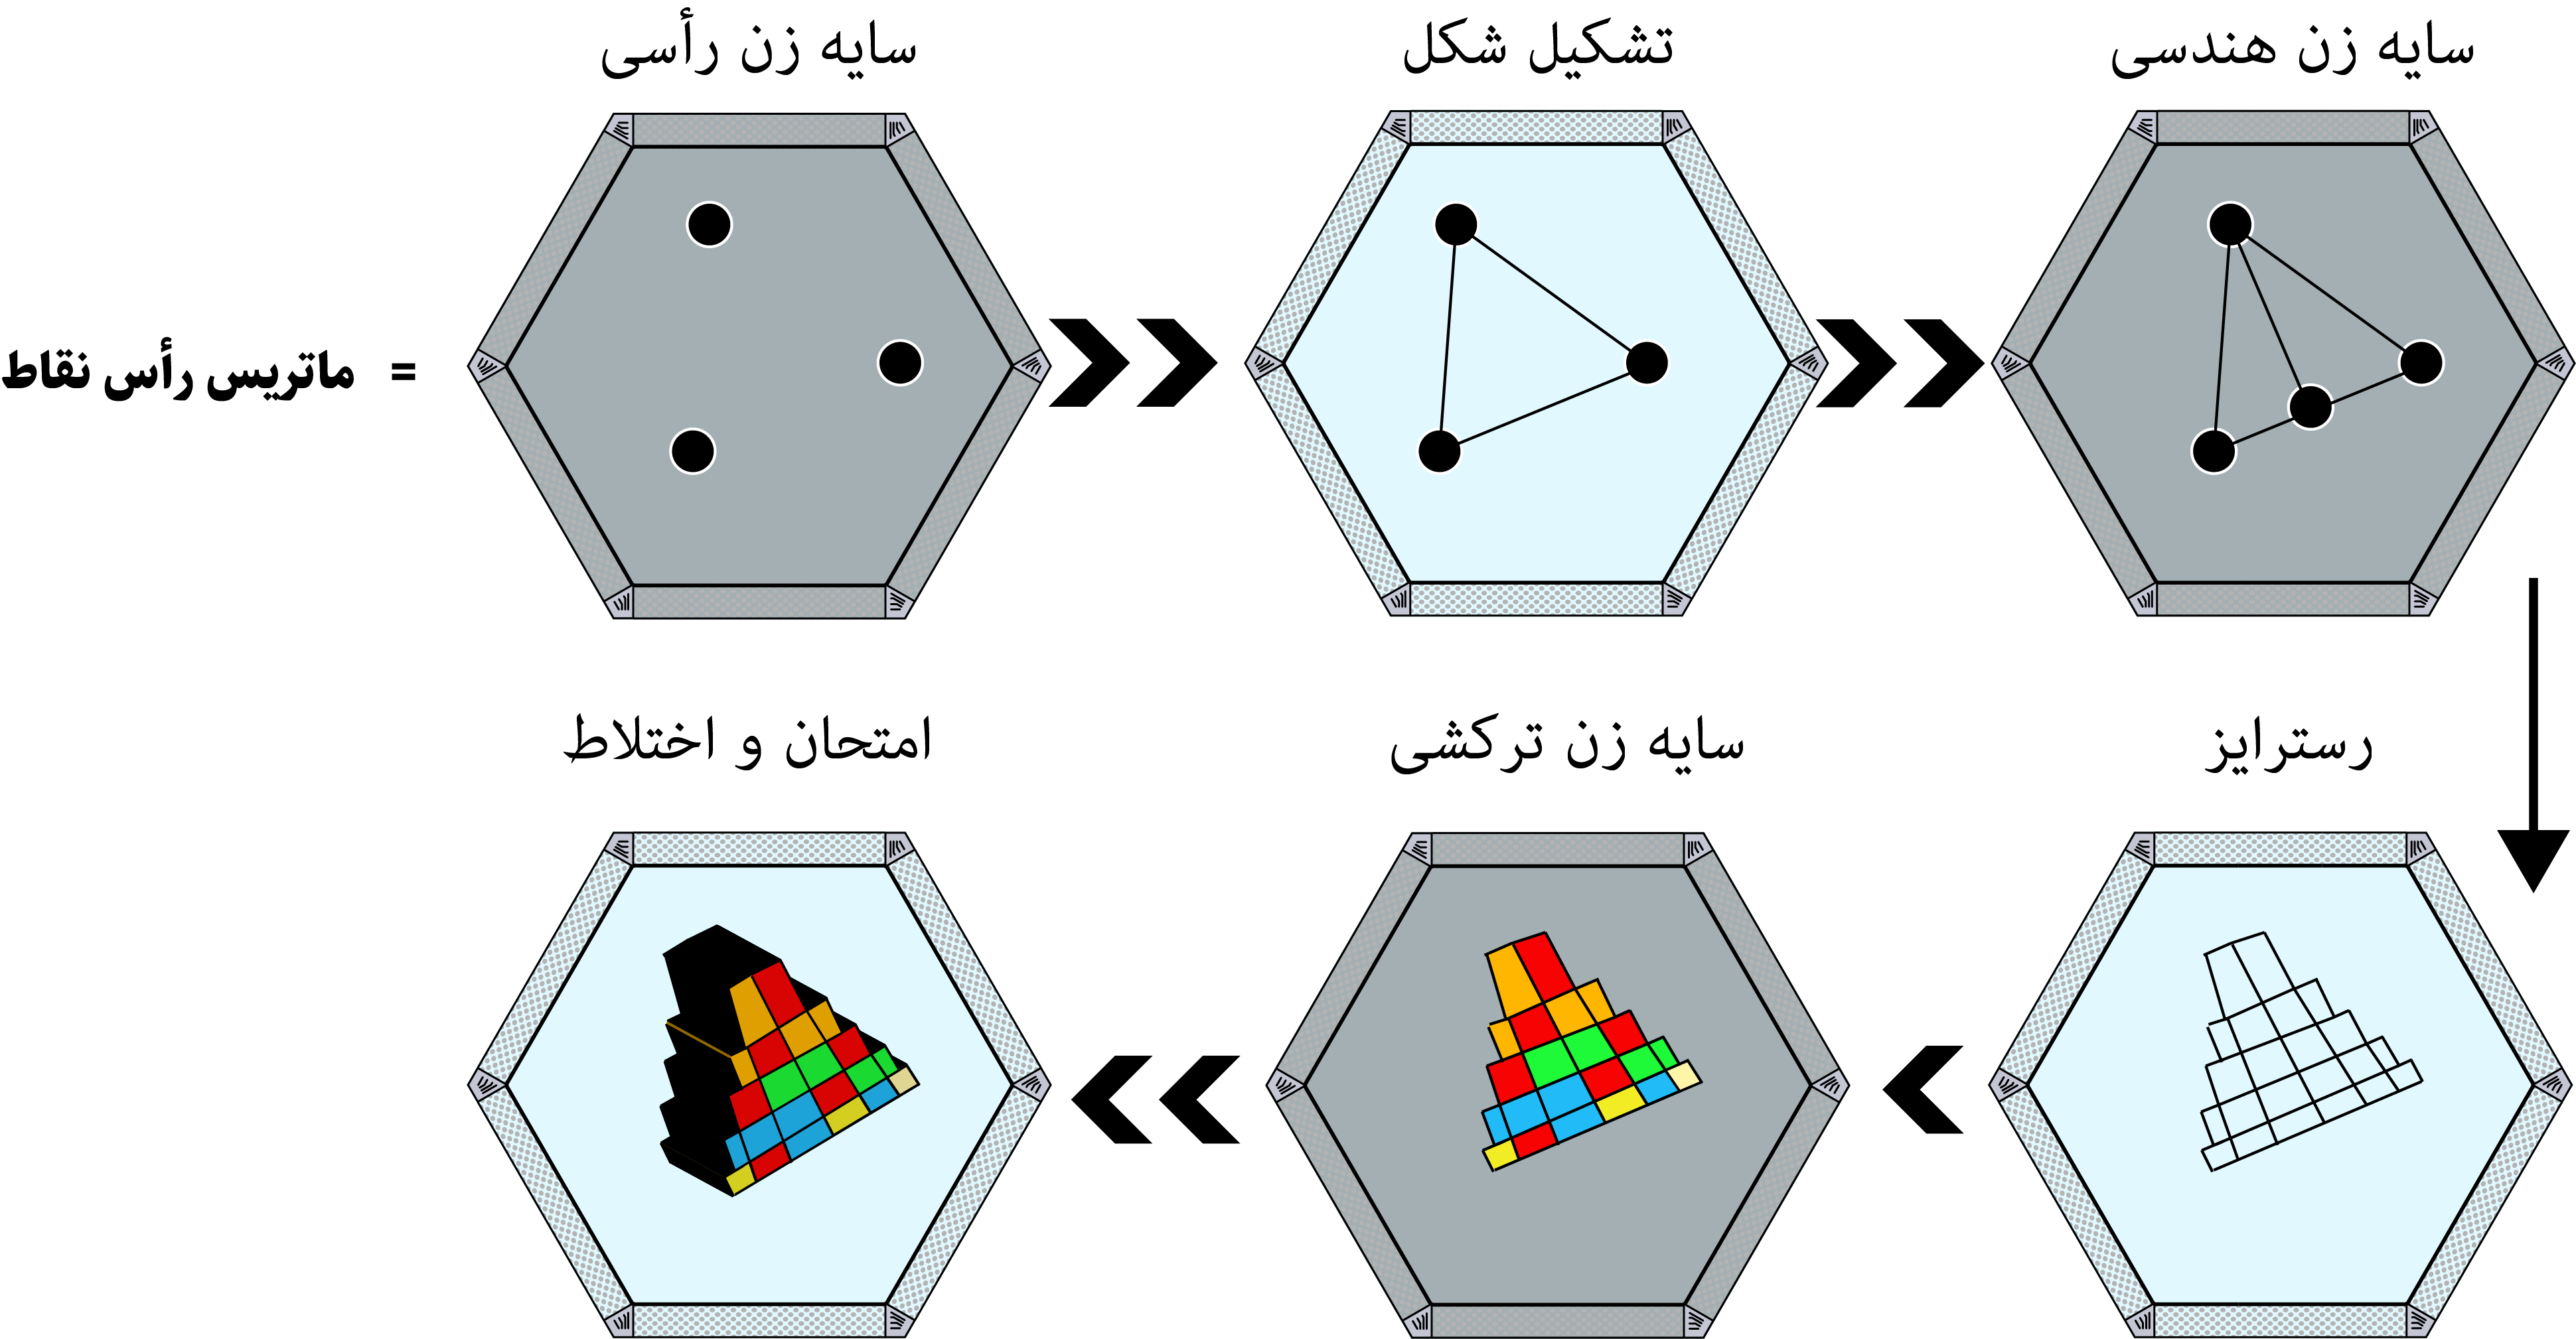
\includegraphics[scale=0.4]{Pipeline}
	 	\caption{خط لوله گرافیکی اوپن جی ال}
	 \end{figure}
	 
	 
	 گروه Kronos همچنین یک رابط نرم افزاری دیگر اعلام میدارد که \textbf{OpenCL} --- با C --- نام دارد. این رابط نرم افزاری به کاربر اجازه میدهد سایه زنها را روی پراسسور مرکزی اجرا کند. به این سایه زنها \textbf{مغزک}\footnote{Kernel} میگویند. شرکتهای زیادی با استفاده ازین رابط نرم افزاری، خط لوله ها وابسته به پراسسور مرکزی خود را میسازند و به عنوان رندرر برای پکیجهای سه بعدی عرضه میدارند. همچنین گاهی میتوان با غیرفعال کردن بخشی از خط لوله، به اثراتی خاص دست یافت. مثلا اثر \lr{\textbf{Cel Shading}} که با دستکاری بخش اختلاط به دست می آید.
	 
	\begin{figure}[H]
		\centering
		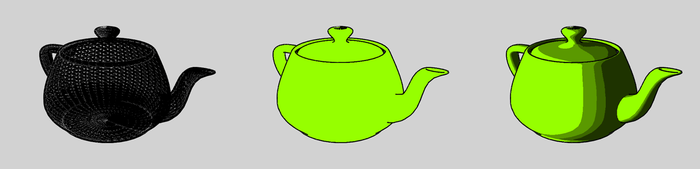
\includegraphics[scale=0.3]{Cel}
		\caption{سایه زنی سلولی}
	\end{figure}
	 
	 
	 \section{فریم بافر و وی رم}\label{vram}
	 
	 
	 \begin{figure}[H]
	 	\centering
	 	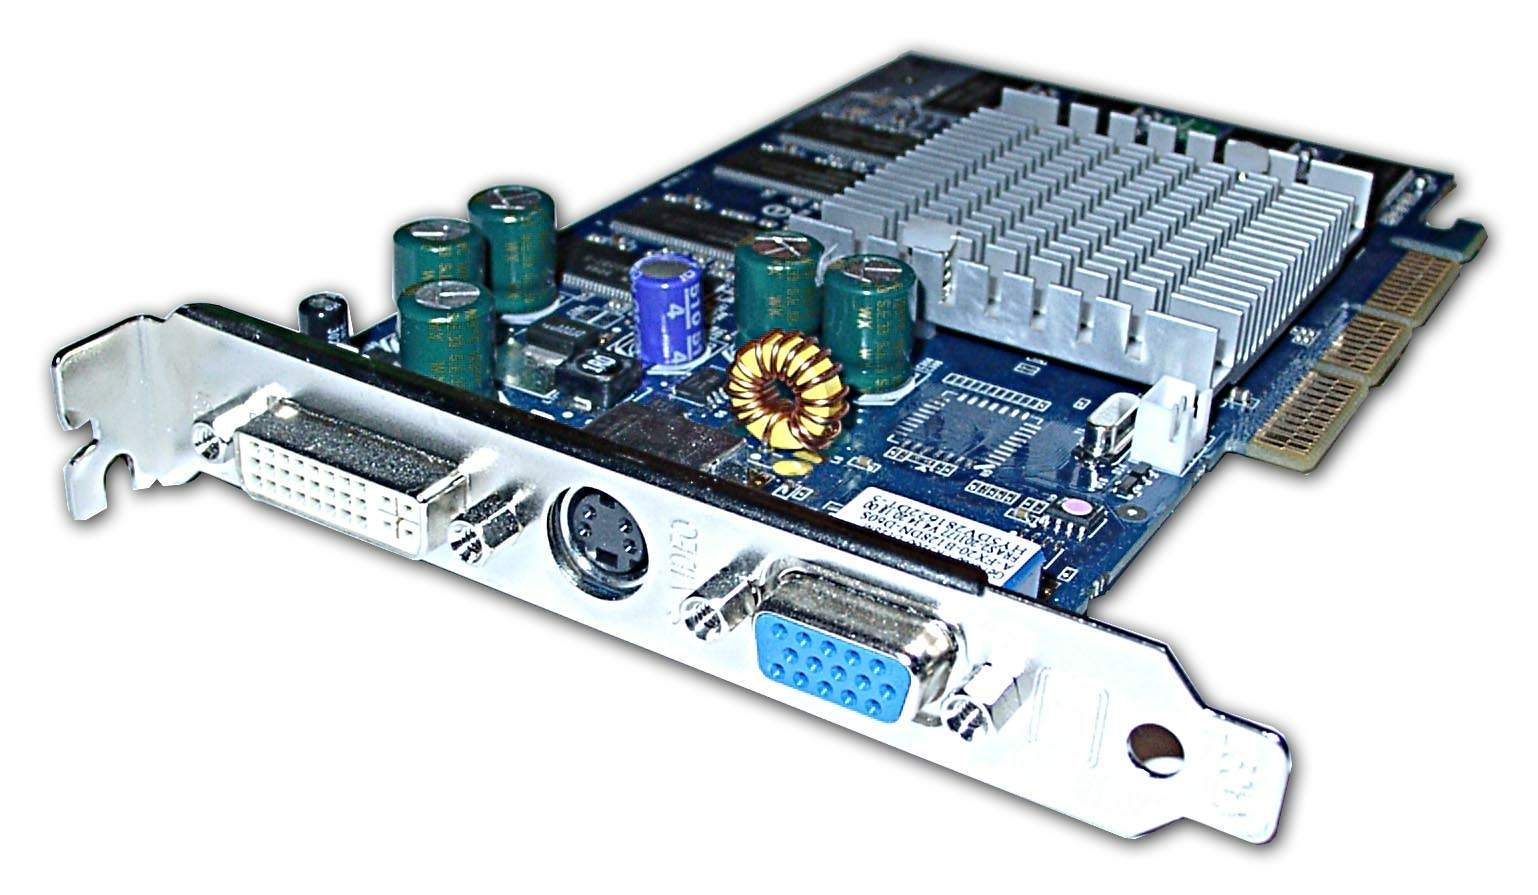
\includegraphics[scale=0.3]{5200}
	 	\caption{GeForce 5200 FX}
	 \end{figure}
 
 در تصویر بالا، اولین کارت گرافیک مرا میبینید. آن زمان، این کارت گرافیک با اینکه حافظه ی ویدئویی بالایی داشت، بازهم ضعیف بود چون کلاک پراسسورش کم بود. خیلی از مردم گمان میکنند حافظه ی گرافیکی، یا \textbf{VRAM} تعیین کننده ی قدرت کارت گرافیک است. درحالی که حافظه ی گرافیکی تنها نگه دارنده ی مرحله ی آخر خط لوله ی گرافیکی، یعنی \textbf{فریم بافر}\footnote{\lr{Frame Buffer}} است.
 
 هنگامی که سایه زن ترکشی کارش تمام شده، و اختلاط صورت میپذیرد، تمام فریمهایی که رسترایز شده اند، وارد حافظه ی ویدئویی میشوند. به این مرحله، همانطور که گفتیم، فریم بافر میگویند.
 
 \begin{figure}[H]
\centering

\includegraphics[scale=0.9]{FrameBuffer}
\caption{تمثیل فریم بافر}
 \end{figure}
	 
	 
	 
	 
	 در کامپیوترهای قدیمی فریم بافر جزئی از رم بود. اما امروزه وی رم جزئی از کارت گرافیک است. فریم بافر، فاصله ی بین پراسسور گرافیکی و پراسسور مرکزی میباشد. در مورد فریم بافر بیشتر صحبت خواهیم نمود.
	 
	 
	 
	 \section{ پایان فصل مفهومات گرافیکی}
	 
	 به پایان فصل مفهومات گرافیکی رسیدیم. مفاهیمی که آموختیم، پایه بود و تنها به عنوان یک سکوی پرتاب حساب میشود. در فصلهای بعدی در مورد اوپن جی ال و سایه زنها خواهیم آموخت. قبل از جهش به فصل بعد، سعی کنید تمام مفاهیمی که آموختیم را در اینترنت جست و جو کرده، و بیشتر در مورد آنها بیاموزید. در بخش \ref{draw} در مورد الگوریتمهای رسم و منحنیهای گرافیکی خواهید خواند.
	 
	 
	 
	 \chapter{الگوریتمهای رنگ، رسم و منحنیها}\label{draw}
	 
	در این فصل، در مورد الگوریتمهای رسم اشکال هندسی در صفحه ی رستر، رنگ، و رسترایز کردن ساده، حرف خواهیم زد. کدهای این فصل نام گذاری شده اند و در فایل \textbf{codes.zip} که از سایت خریده اید، حاظر و آماده ی کپی کردن هستند.
	
	
\begin{files}
	اکثر کدهایی که در این کتاب میبینید نوشته ی خود من هستند، و خواهشا وقتی انها را جای دیگری پست میکنید، از من نام ببرید و لینک کتاب را اضافه کنید. 
\end{files}


اما قبل از آن، برای تست الگوریتمایمان، احتیاج به یک پکیج رستر داریم. ما برای این امر از پکیج رستر \textbf{Pillow} پایتان استفاده مینیم. اما قبل از آن بگذارید رنگ در کامپیوتر را توضیح بدهم.

\section{رنگ  در کامپیوتر}\label{color}

گفتیم سایه زن های ترکشی، به پیکسلها، رنگ میدهند. اما این رنگ چگونه حساب میشود؟ برای اینکار باید به تاریخ بازگردیم. زمانی که فلاسفه ی یونیه مانند ارسطو باور داشتند رنگ، موهبتی از خدایان است و از چهار عنصر آتش، خاک، باد، و آب تشکیل شده است.

\begin{figure}[H]
	\centering
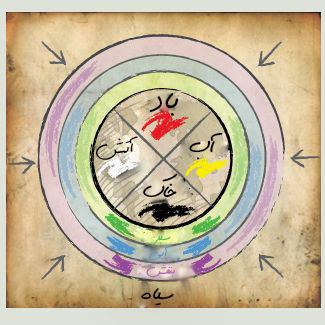
\includegraphics[scale=1]{GreekColor}
\caption{تصور ارسطو از رنگ}
\end{figure}


در سال 1666 آیزک نیوتون نشان داد که میتوان با رد کردن رنگ از بین دو \textbf{منشور}\footnote{Prism} یک طیف رنگی --- که مساوی رنگهای رنگین کمان است --- به دست آورد.

\begin{figure}[H]
	\centering
	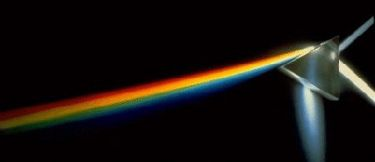
\includegraphics[scale=1]{Prism}
	\caption{طیف رنگی}
\end{figure}

میتوان با داغ کردن یک اتم هیدروژن، نور ساطع شده از آن را با همین تکنیک، شکست. به این نور شکسته شده، \textbf{طیف نشری خطی}\footnote{\lr{Emission Spectrum}} هیدروژن، یا هر اتم دیگری، میگویند.


\begin{figure}[H]
	\centering
	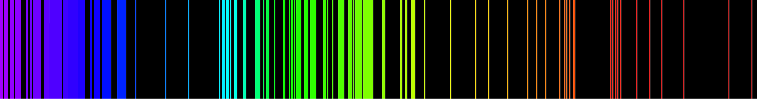
\includegraphics[scale=0.4]{IronSpectrum}
	\caption{طیف نشری خطی آهن}
\end{figure}


در دنیای واقعی، رنگها از قرمز، آبی، و زرد تشکیل شده اند. اما در مانیتورهای امروزی، این سه رنگ، قرمز، سبز، و آبی میباشد. از زمان خروجی آرائه ی ویدئوگرافیکی تا به الان، \textbf{فضای رنگی}\footnote{Colorspace} ای که سایه زنها استفاده میکردند، فضای \textbf{"قرمز سبز آبی "} یا RGB میباشد. 



\begin{figure}[H]
	\centering
	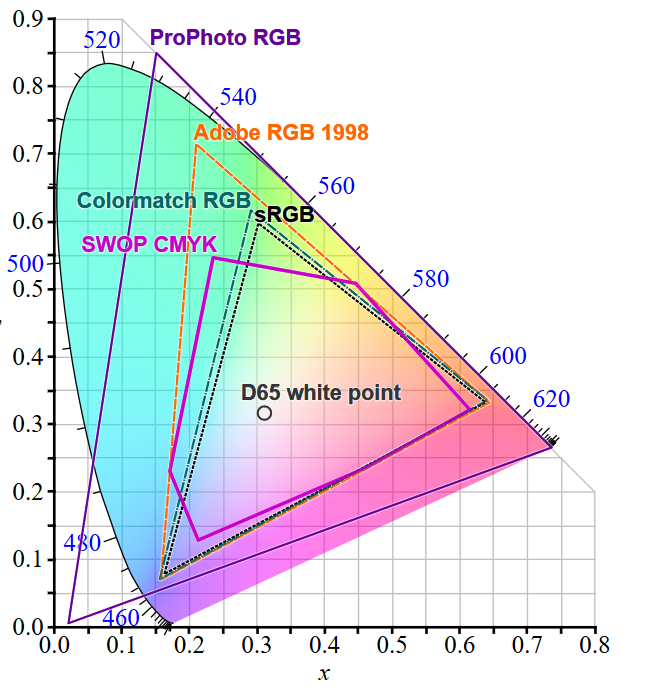
\includegraphics[scale=0.6]{RGBModel}
	\caption{فضای قرمز، سبز، آبی در دستگاه مختصات دکارتی}
\end{figure}

همانطور که مشاهده میکنید، RGB یک فضای مثلت تا نیم دایره مانند، بسته به ورژن آن، در صفحه ی مختصات دکارتی میباشد. هررنگ در فضای RGB به صورت یک تاپل سه عددی \lr{(r, g, b) } نمایش داده میشود. هرکدام ازین سه، بین 0 تا 255 قرار دارد. میتوانید با آنا بالای 16 میلیون رنگ بسازید. اگر این اعداد را \textbf{نرمال سازی}\footnote{Normalize} کنیم بین 0 و 1 میشوند. و سایه زن ها ازین اعداد استفاده میکنند. 

در کامپیوتر جز RGB  --- که در فضای مختصات دو بعدی قرار دارد --- ما میتوانیم از مدلهای رنگ و فضاهای رنگ دیگر نیز استفاده کنیم. یکی ازین مدلها و فضهاها، \textbf{ته رنگ، اشباع، ارزش }\footnote{\lr{Hue, Saturation,  Value}}  یا HSV نام دارد که یک استوانه در دستگاه مختصات قطبی میباشد.

 \begin{figure}[H]
 	\centering
 	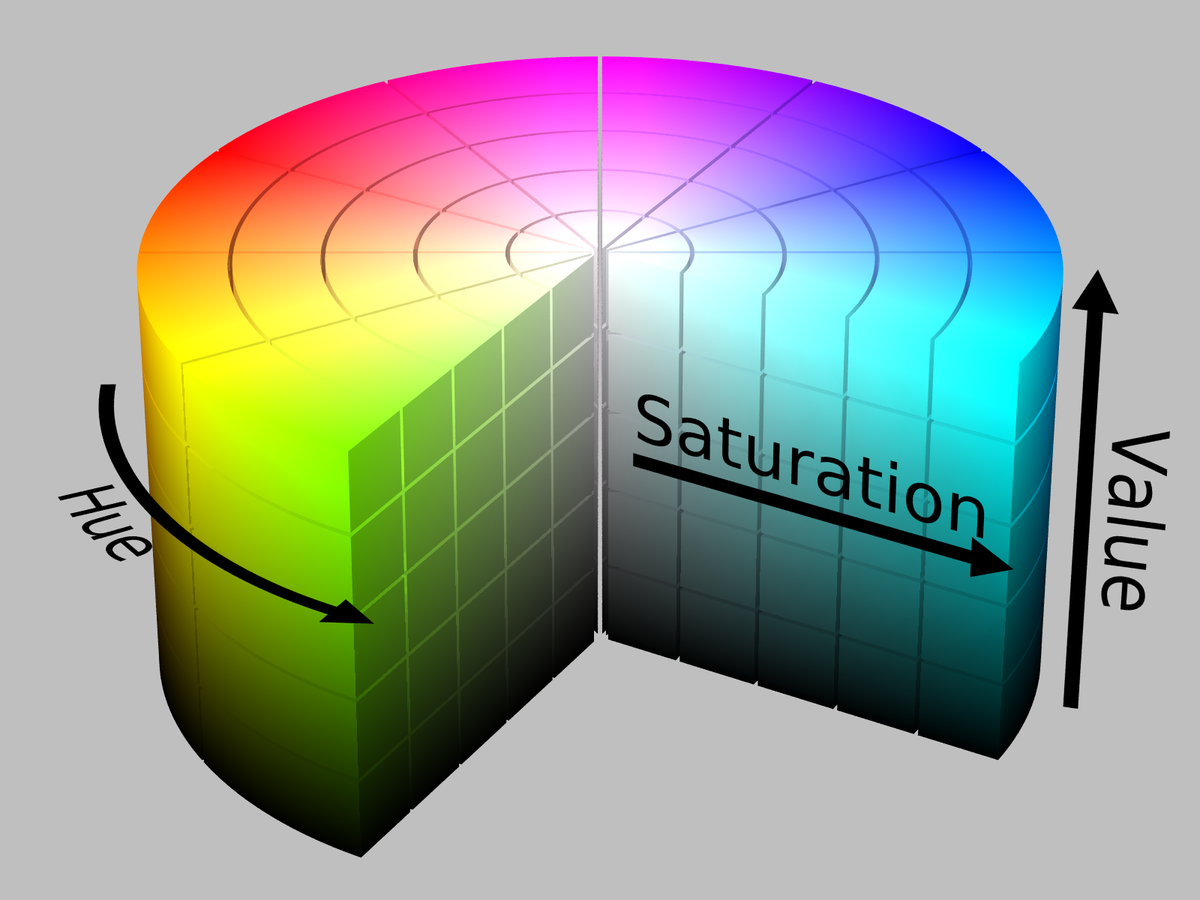
\includegraphics[scale=0.3]{HSVModel}
 	\caption{فضای ته رنگ، اشباع، ارزش در دستگاه مختصات قطبی }
 \end{figure}

رنگهای این فضا به صورت یک تاپل \lr{(h, s, v)} نمایش داده شده، و هرکدامشان اعداد درصدی بین 0 و 100 هستند. 

هم RGB و HSV یک عضو چهارم به نام \textbf{اَلفا} دارند که نشان دهنده ی پررنگی  یا کمرنگی رنگ است.


میتوان با استفاده از پکیج colorsys پایتان، که به صورت معمول روی همه ی عرضه های اینترپرتر نصب است، رنگها را از بین فضاهای مختلف تبدیل کرد. بعدا ازین تکنیک استفاده خواهیم نمود.





\section{کتابخانه ی تصویری پایتان}
	
	کتابخانه ی تصویری پایتان در قدیم PIL نام داشت و همراه پکیجهای اصلی عرضه میشد. اما، از ورژن 3 ببعد، آپدیت این پکیج قطع گردید و ما هم اکنون برای استفاده از آن مجبوریم از پکیج Pillow که یک \textbf{کد کاغذ کادویی}\footnote{Wrapper} از PIL میباشد استفاده نماییم.
	
	همانطور که آموزش دادیم، با استفاده از پیپ --- pip --- پکیج Pillow را نصب کنید. سپس به حالت زیر عمل کنید:
	
	
	
	
		 	 	 	 \begin{latin}
		\mono{	\begin{lstlisting}[backgroundcolor = \color{lightgray},caption={PIL-Intro.py},captionpos=b]

from PIL import Image

img = Image.new('RGB', (32, 32), color= 'red')
img.save('pil_color.png')

			\end{lstlisting}}	 
		
	\end{latin}
	
	
	اگر عکسی که ایجاد میشود (در فولدر کد) را باز کنید، عکس زیر را خواهید دید:
	
	\begin{figure}[H]
		\centering
		
\includegraphics[scale=1]{RedImage}		
		\caption{تصویر 32 در 32 پیکسل رستر ما}
	
	\end{figure}

اینگونه یک تصویر 32 در 32 ایجاد میکنیم. میتوانید سایز، و رنگ را تغییر بدهیم.
	
	
	
			 	 	 	 \begin{latin}
		\mono{	\begin{lstlisting}[backgroundcolor = \color{lightgray},caption={PIL-ChangeColor.py},captionpos=b]
			
img = Image.new('RGB', (64, 64), color= (23, 11, 24))
img.save('pil_ChangedColor.png'))
			
			\end{lstlisting}}	 
		
	\end{latin}
	
	فایل جدید را باز کرده، و متوجه خواهید شد که یک تصویر 64 در 64 خواهید دید. 
	میتوان اطلاعات پیکسل خاص را تعیین کرد، و یا اطلاعت پیکسل خاص را ااز رستر گرفت.
	
	
	
				 	 	 	 \begin{latin}
		
		\mono{	\begin{lstlisting}[backgroundcolor = \color{lightgray},caption={PIL-GetSet.py},captionpos=b]
pixels = img.load()
print(pixels[32, 32]) #get
pixels[32, 32] = (255, 255, 255) #set
print(pixels[32, 32]) #get again
			
			
img.save('pil_GetSet.png')
			\end{lstlisting}}	 
		
	\end{latin}
	
	
	این یک تصویر مشکی با یک نقطه ی سفید در وسطش تولید میکند. همانطور که میبینید کافیست نقطه ای که میخواهیم را بین آکولاد قرار داده و رنگی که میخواهیم به صورت تاپل سه تایی به پیکسل میدهیم.
	
	 
همچنین میتوانیم یک یک \textbf{گرادیان}\footnote{Gradient} 
	
	
	
	
	
	
	
	
	
	
	
	
	
	
	
	
	
	
	
	
	
	
	
	
	 
	 
	 
	 
	 
\end{document}